\chapter{Technische Umsetzung} \label{implementation}

Die technische Umsetzung befasst sich mit der Implementation der aus dem Lösungsdesign gewonnenen Erkenntnisse. Dazu werden die vorgestellten Prinzipien des Software-Designs und der Algorithmus umgesetzt. Hierfür werden diese konkret in \gls{Typescript} programmiert und innerhalb der Applikationsstruktur platziert. Diese Struktur basiert zum einen auf dem bestehenden \gls{ikc-core} und zum anderen auf der vorgestellten Struktur innerhalb des \hyperref[arcitecture]{\textit{Kapitels der Architektur}}. Punktuell wird die Implementation zusätzlich durch die Nutzung von verschiedenen externen \gls{Bibliothek}[en] optimiert.

Die gezeigten Code-Ausschnitten werden bei Bedarf für dieses Dokument angepasst. Diese Änderungen dienen der Verständlichkeit im Kontext des Dokuments und beinhalten lediglich strukturelle, jedoch keine Änderungen an der Applikationslogik.



% -------------------------------


%    \begin{figure}[H]
%    \centering
%    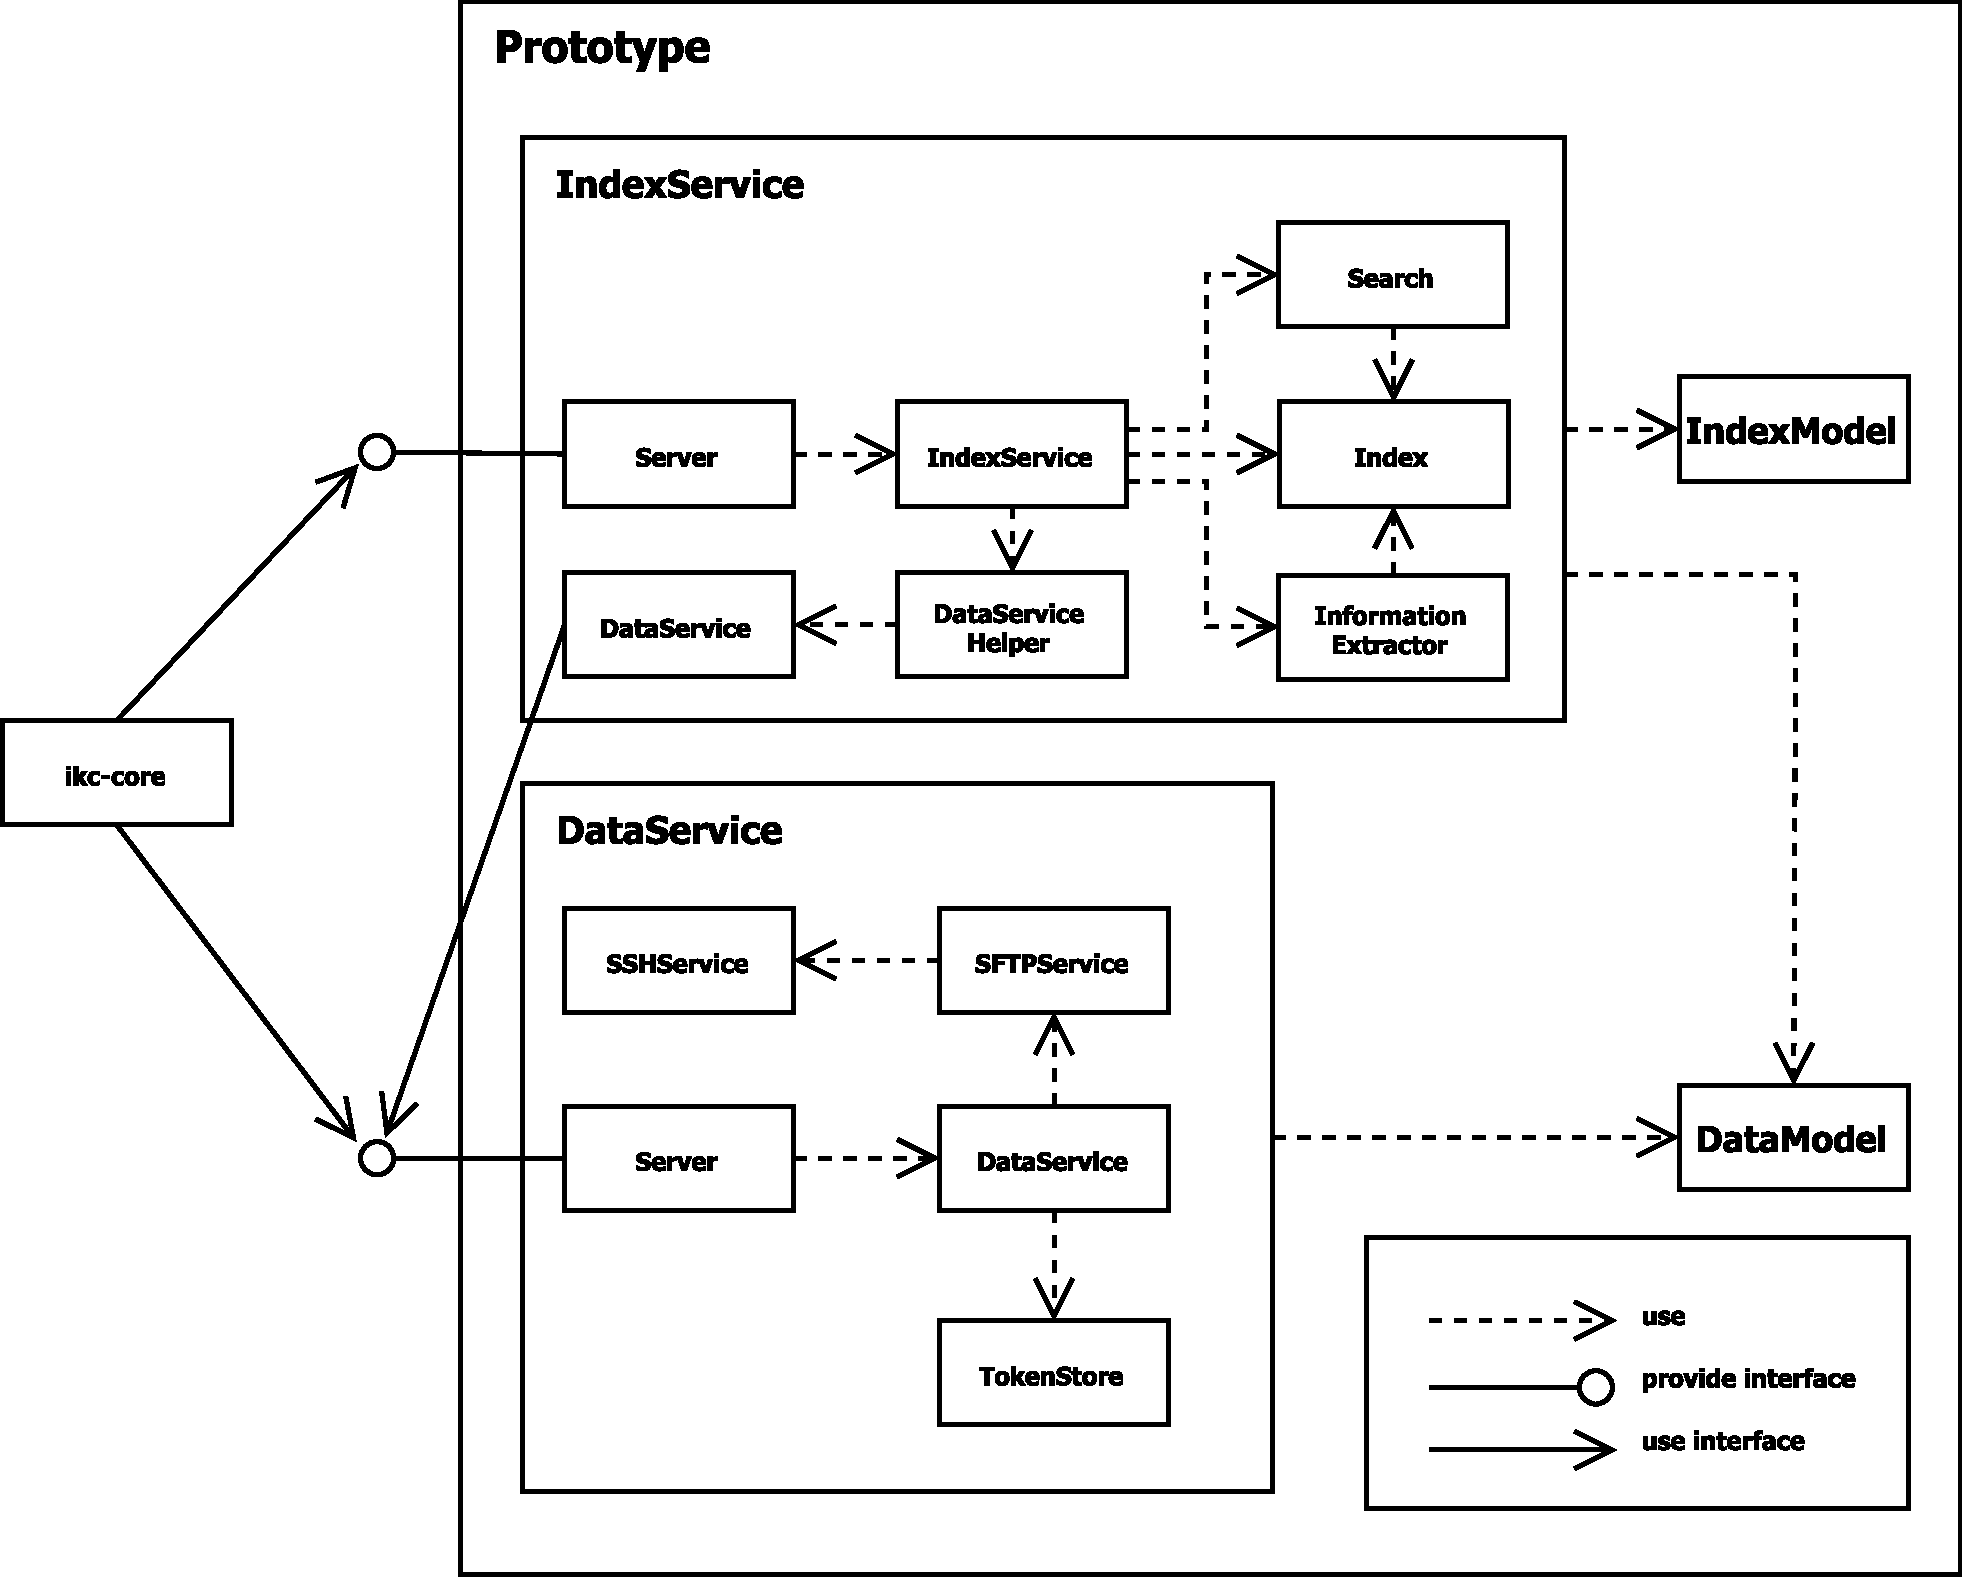
\includegraphics[width=1\textwidth]{PrototypeClassDiagram}
%    \caption{Prototype Klassendiagram}
%    \label{fig:prototypeClassDiagram}
%    \end{figure}

Der Kern der Software bildet der Algorithmus, dieser ist, neben der Suchfunktionalität und dem Aufbau der Indizes, ein Hauptbestandteil des \texttt{IndexService}. Der \autoref{indexservice} gewährt einen Überblick über die beteiligten Komponenten und deren ungefähre Funktionalität. Als Grund\-la\-ge benötigt der \texttt{In\-dex\-Ser\-vice} alle zu indexierenden Dateien im Volltext. Deren Quelle ist der \texttt{Data\-Ser\-vice}. Der \texttt{Index-} und der \texttt{Da\-ta\-Ser\-vi\-ce} bilden zusammen den eigentlichen Prototypen. Eine kurze Einführung folgt in den folgenden Abschnitten. Er\-wähn\-ens\-wer\-te weitere Themen in diesem Kapitel ist der Umgang mit Daten und die Kommunikation zwischen den verschiedenen Servies. Wie in der Bausteinsicht auf \autoref{fig:bausteinsicht} zu erkennen, gibt es neben der Integration der Services auch eine Einbindung in die bestehende Benutzeroberfläche des \gls{ikc-core}.

% Folgend zunächst eine kurze Erklärung zu den einzelnen Klassen des \texttt{Index-} beziehungsweise \texttt{DataServices}.

\newpage

\section{IndexService}\label{indexservice}

Innerhalb des \texttt{IndexService} werden die primären Funktionen des Prototyps für die Schlüsselwort-Extraktion gekapselt. \autoref{fig:indexserviceClassDiagram} zeigt dabei, wie die wichtigsten Klassen miteinander kommunizieren. Anschliessend werden zentrale Abläufe genauer belichtet. 

    \begin{figure}[H]
    \centering
    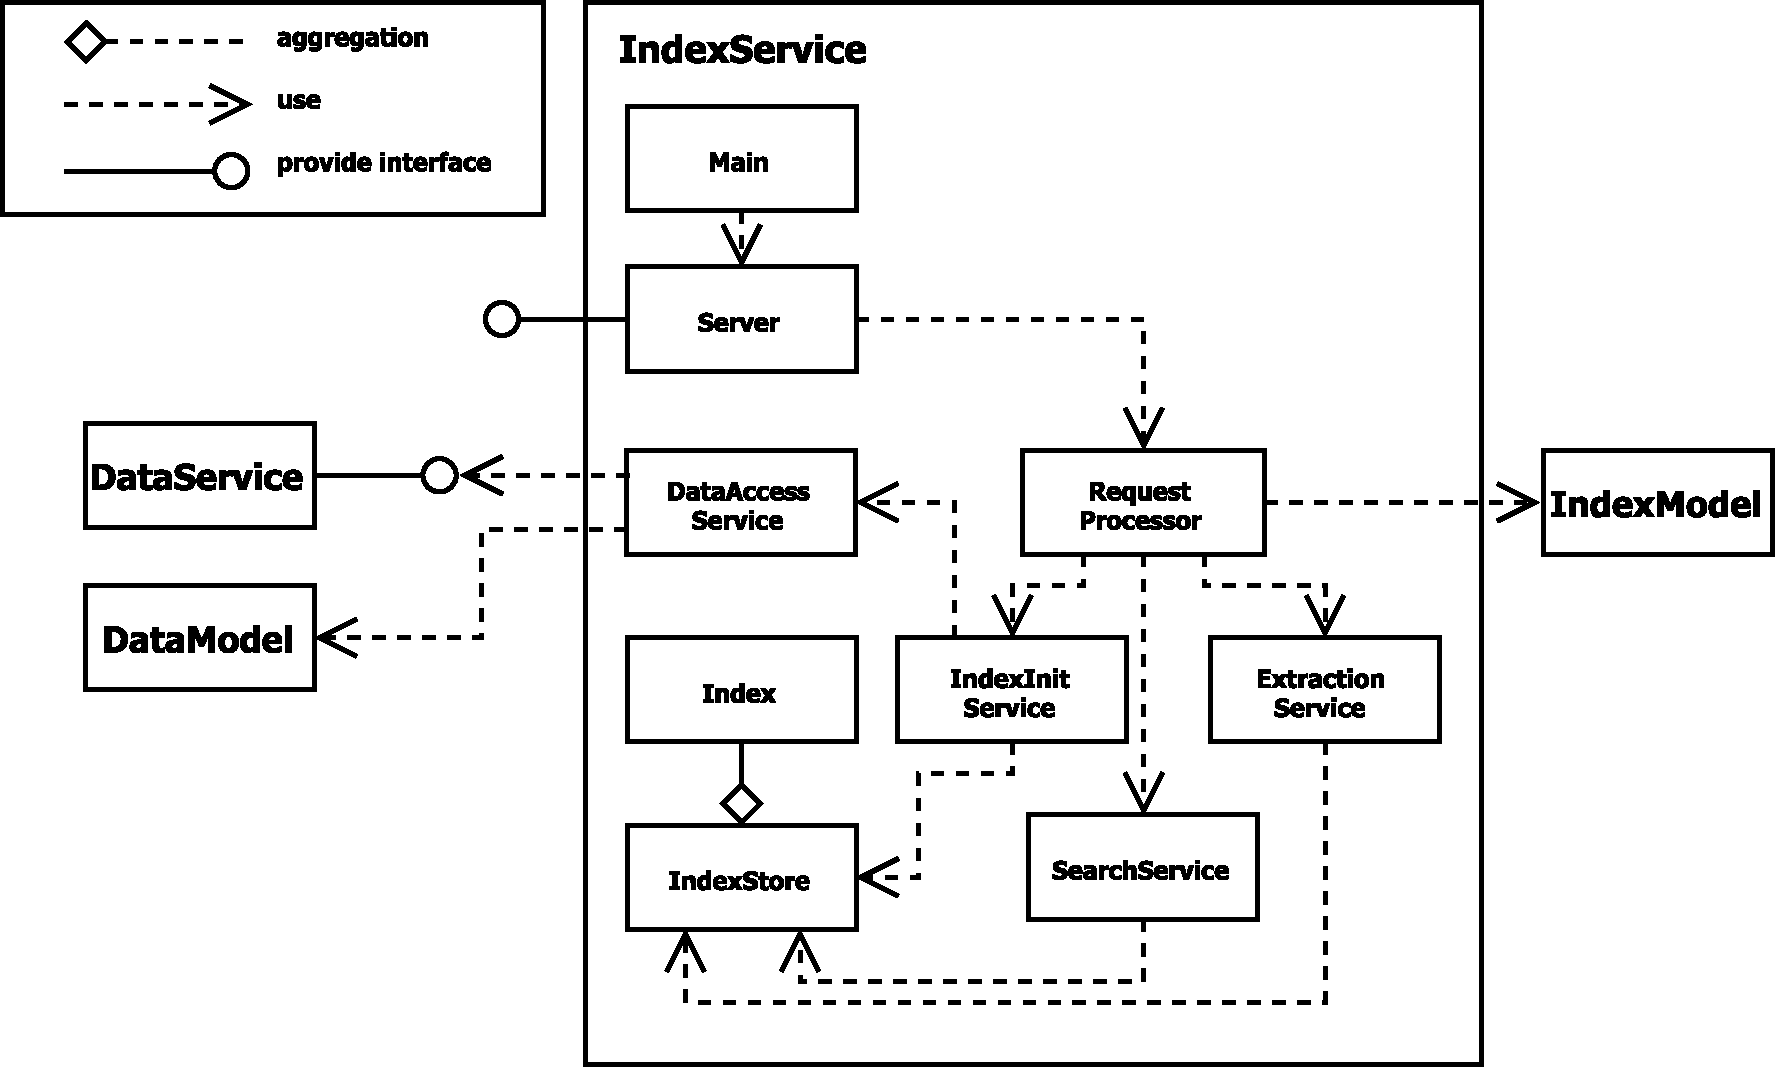
\includegraphics[width=1\textwidth]{IndexServiceClassDiagram}
    \caption{IndexService Klassendiagram}
    \label{fig:indexserviceClassDiagram}
    \end{figure}

\begin{itemize}
    \item \textbf{Main}: Die Klasse \texttt{Main} ist die zentrale Starter Klasse des ganzen Service. Dazu initialisiert sie den Server. 
    \item \textbf{Server}: Hier werden Netzwerk-Anfragen entgegengenommen. Und gegebenenfalls wird eine Antwort zu\-rück\-ge\-schi\-ckt.
    \item \textbf{Index}: Das Datenobjekt \texttt{Index} bietet alle Daten, welche für die Suche als auch für die Extraktion von \gls{Keyword}[s] und Dokumenten benötigt werden. Diese Klasse wird jedoch zur reinen Datenhaltung verwendet und beinhaltet keinerlei implementierte Logik. Sie beinhaltet den Volltext Index und den Frequenz Index. 
    \item \textbf{MessageManager}: Dies ist der Kern des \texttt{IndexService}: Anfragen werden basierend auf deren Type auf die drei Services \texttt{Search\-Ser\-vi\-ce}, \texttt{ExtractionService} und \texttt{IndexInitService} zur Verarbeitung weitergeleitet.
    \item \textbf{IndexInitService}: Die Aufgabe einen \texttt{Index} zu laden hat der \texttt{IndexInitService}, dazu kann er über den \texttt{DataAccessService} auf den \texttt{DataService} zugreifen um die benötigten Daten abzufragen. Nach der Initialisierung wird der entsprechende \texttt{Index} innerhalb des \texttt{IndexStore} abgelegt.
    \item \textbf{SearchService}: Dieser Service ist verantwortlich für die Abarbeitung von Suchanfragen. Als Grundlage für die Resultate wird der Volltext Index verwendet.  
    \item \textbf{ExtractionService}: Die Extraktion von \gls{Keyword} oder Dokumenten wird durch den \texttt{ExtractionService} erledigt. 
    \item \textbf{DataAccessService}: Fungiert als Schnittstelle zum \texttt{DataService}.
    \item \textbf{IndexStore}: Beinhaltet alle geladenen \texttt{Index} Objekte und stellt diese zu Verfügung. 
\end{itemize}

\subsection{Integration des Algorithmus}\label{impalgo}
Der vorgestellte Algorithmus wird innerhalb des \texttt{IndexService} in der Klasse \texttt{ExtractionHelper} implementiert. Sie stellt zwei Methoden mit denen relevante \gls{Keyword}[s] (\texttt{getKeywordsForDocument}) oder relvante Dokumente (\texttt{getDocumentsForKeyword}) berechnet werden können. Da sie Funktionen bereitstellt, jedoch selbst keine Eigenschaften beispielsweise in Form von Variablen hält, muss ihr der benötigte Index mit der aufgerufenen Funktion zu Verfügung gestellt werden. 
Folgend wird die Implementation der verschiedenen Schritte des Algorithmus genauer erläutert.

\subsubsection{Vorverarbeitung}
Im ersten Schritt geht es um die Vorverarbeitung des Texts. Dazu wird \gls{regex} verwendet, dadurch kann die Grösse des Codes erheblich reduziert werden im Vergleich zu einer Implementation ohne \gls{regex}. \autoref{preprocessing} zeigt die zwei nötigen Schritte:
\begin{itemize}
    \item Zuerst wird der Buchstabe welcher auf einen Punkt, Fragezeichen, Ausrufezeichen oder Zeilenschaltung folgt in die Kleinschreibung umgewandelt. Mithilfe des \gls{regex} Ausdrucks werden diese erkannt und mittels einer anonymen Funktion transformiert.
    \item Anschliessend werden die einzelne Fragmente des Textes gebildet. Dazu wird ein \gls{regex} Ausdruck verwendet, welcher eine Kollektion von Text Fragmente zurückgibt. Anders als bei dem vorherigen Schritt, wird eine Negation innerhalb des Ausdrucks verwendet. Dadurch werden nur Text Fragmente ausgewählt welche die entsprechenden Zeichen nicht enthalten. Somit enthält ein Fragment den Text zwischen einem Punkt und einem Komma oder innerhalb zweier Klammer. 
\end{itemize}

\begin{listing}[H]
\inputminted[
frame=lines,
framesep=2mm,
baselinestretch=1.2,
linenos,
breaklines=true
]{js}{sourcecode/IndexService/ExtractionHelper/processtext.ts}
\caption{Vorberarbeitung}
\label{preprocessing}
\end{listing}

\subsubsection{Text Zerlegung}
Die Text Fragmenten werden nun in die verschiedenen Wörter zerlegt. \autoref{listing:tokenization} zeigt die nötigen Schritte dazu:
\begin{itemize}
    \item Alle Fragmente werden bei einem Leerschlag aufgesplitet (Zeile 3).
    \item weiter werden "'s " durch " " ersetzt (Zeile 6).
    \item Anschliessend werden unerwünschte Sonderzeichen zu Beginn oder am Ende eines Wortes mithilfe der Funktion \texttt{trimmer} der \gls{elasticlunr} Bibliothek entfernt (Zeile 5).
    \item Zum Schluss werden leer Wörter gefiltert um diese nicht weiter zu verarbeiten (Zeile 9-11). 
\end{itemize}

\begin{listing}[H]
\inputminted[
frame=lines,
framesep=2mm,
baselinestretch=1.2,
linenos,
breaklines=true
]{js}{sourcecode/IndexService/ExtractionHelper/tokenization.ts}
\caption{Text Zerlegung}
\label{listing:tokenization}
\end{listing}


\subsubsection{Generierung möglicher Keywords}
Für die Generierung möglicher \gls{Keyword}[s] werden drei verschachtelte Schlaufen verwendet. Die äusserste (Zeile 2) iteriert über die einzelnen Fragemente, die mittlere (Zeile 4) über die einzelnen Wörter innerhalb eines Text Fragment und die innere (Zeile 12) über die Länge der \gls{N-Gramm}[e] von eins bis \texttt{n}.
\autoref{generatekeywords} zeigt den genaueren Ablauf und in \autoref{fig:exampleloop} ist ein genaueres Beispiel der drei Schlaufen ersichtlich:
\begin{itemize}
     \item Falls eine \gls{N-Gramm} länger als die verbliebenen Anzahl Wörter innerhalb des Fragments ist, muss die maximale Länge Reduziert werden. So zum Beispiel wenn noch zwei Wörter übrig bleiben können nur noch \textit{2-Gramme} und \textit{1-Gramme} gebildetet werden und die Länge muss auf \texttt{length = 2} reduziert werden. (Zeile 6-9)
     \item Um die \gls{N-Gramm}[e] zu generieren werden nun eine List von Wörter aus dem Fragement ausgelesen. Dies Mithilfe der Methode \texttt{slice} und anschliessend mit \texttt{join} als Begriff zusammengeführt. Beide Methoden sind Teil der Standard \texttt{Array} Klasse von Typescript. (Zeile 13-14)
     \item Schlussendlich werden nun die generierten \gls{N-Gramm}[e] (\gls{Keyword}[s]) in einer Map zusammen mit ihrer Häufigkeit gespeichert.
\end{itemize}

\begin{listing}[H]
\inputminted[
frame=lines,
framesep=2mm,
baselinestretch=1.2,
linenos,
breaklines=true
]{js}{sourcecode/IndexService/ExtractionHelper/generate-keywords.ts}
\caption{Keywords Generierung}
\label{generatekeywords}
\end{listing}

\begin{figure}[H]
\centering
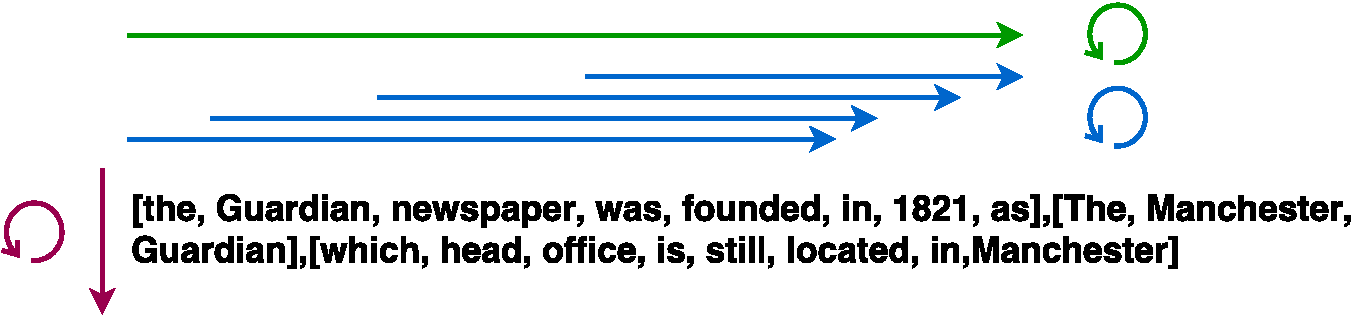
\includegraphics[width=1\textwidth]{exampleloop}
\caption{Beispiel Schlaufe}
\label{fig:exampleloop}
\end{figure}



\subsubsection{Filter mittels POS Tagger}
Bevor die Relvanz der \gls{Keyword}[s] berechnet werden können werden sie ein weiteres reduziert mithilfe eines Filters basierend auf dem POS Tagger. Dazu zeigt \autoref{filter} die nötigen Schritte.
\begin{itemize}
    \item Für jedes mögliche \gls{Keyword} werden die Wortarten der einzelnen Wörter berechnet. Dies wird mittels der Methode \texttt{tag} aus der externen Bibliothek \textit{js-pos} durchgeführt. Als Resultat wird eine \texttt{Array} zurückgegeben, welches für jedes Wort wiederum eine \texttt{Array} enthält mit dem Wort und der Wortart. Neben dem Wort auch zum Beispiel die Zeit eines Verbs oder der Numerus eines Nomens erkannt. Innerhalb der Dokumentation der Bibliothek ist eine Liste mit allen möglichen Resultaten angefügt. Anschliessend wird das jeweilige \gls{Keyword} mithilfe der drei Methoden \texttt{properNGramPos}, \texttt{properNGramStart} und \texttt{properNGramEnd} auf ihre Gültigkeit überprüft. Dies geschieht aufgrund der definierten Vorgaben (\autoref{algo}). \cite{GitHubda36:online} (Zeile 2) 
    \item Als erstes wird überprüft ob das \gls{Keyword} ein Nomen oder ein fremdes Wort enthält. (Zeile 4-13)
    \item Weiter muss das \gls{Keyword} entweder mit einem Nomen, einem Adjektiv, einem fremden Wort oder Grossgeschrieben starten. (Zeile 15-24)
    \item Schlussendlich muss ein gültiges \gls{Keyword} auch mit einem Nomen, einem Adjektiv oder einem fremden Wort enden. (Zeile 26-32)
\end{itemize}

\begin{listing}[H]
\inputminted[
frame=lines,
framesep=2mm,
baselinestretch=1.2,
linenos,
breaklines=true
]{js}{sourcecode/IndexService/ExtractionHelper/filter.ts}
\caption{Filter}
\label{filter}
\end{listing}


\subsubsection{Berechnung der Relevanz}
Der wichtigste Schritt für die Bewertung der einzelnen \gls{Keyword}[s] ist der Berechnete Wert, dies folgt der entsprechenden Formel (\autoref{algo}). Die verschiedenen Schritte werden mithilfe des \autoref{calc} genauer erläutert:
\begin{itemize}
    \item Als erstes muss die Länge des Korpus \texttt{indexLength} berechnet werden. Dies kann direkt aus dem Volltext Index abgefragt werden. Dazu wird die Länge des \texttt{documentStore} berechnet. Anschliessend werden die Anzahl Dokumente \texttt{keywordDocFreq} mit diesem \gls{Keyword} berechnet, dieser Wert kann direkt aus dem Frequenz Index gelesen werden. Zum Schluss muss noch die Anzahl Wörter innerhalb des Dokuments des \gls{Keyword}[s] berechnet werden. (Zeile 2-6)
    \item Basierend auf der Anzahl Dokumenten (\texttt{indexLength}) und der Anzahl Dokumenten mit dem \gls{Keyword} (texttt{keywordDocFreq}) wird als nächstes nun der \textit{idf} Wert (\texttt{keywordIdf}) berechnet. (Zeile 8)
    \item Den \textit{tf} Wert (\texttt{keywordTf}) wird bereits zusammen dem \gls{Keyword} mitgeliefert. (Zeile 10)
    \item Anhand der Dokumentenlänge wird nun eine entsprechende Normierung (\texttt{lengthNorm}) für den Score berechnet. (Zeile 12)
    \item Schlussendlich werden die verschiedenen Wert miteinander multipliziert um den entsprechenden Score zu erhalten. (Zeile 14)
\end{itemize}

\begin{listing}[H]
\inputminted[
frame=lines,
framesep=2mm,
baselinestretch=1.2,
linenos,
breaklines=true
]{js}{sourcecode/IndexService/ExtractionHelper/calc.ts}
\caption{Berechnung Relevant}
\label{calc}
\end{listing}

\subsubsection{Auswahl}
Anschliessend an die Berechnung des Scores wird die Liste mit \gls{Keyword}[s] absteigend sortiert und mit Hilfe eines Schwellwertes begrenzt.

\subsubsection{Dokument Extraktion}
Die entsprechenden Dokumente, welche ein bestimmtes \gls{Keyword} beinhalten, kann direkt aus dem Frequenz Index ausgelesen werden. Dies geschieht durch die folgenden Schritte (\autoref{doc-extraction}):
\begin{itemize}
    \item Mithilfe des \gls{Keyword} können innerhalb des Frequenz Index eine List mit passenden Dokumente abgefragt werden. (Zeile 2)
    \item Anschliessend werden die gleichen Berechnungen wie in \autoref{calc} durchgeführt um die Relevanz der einzelenn Dokumente für das \gls{Keyword} zu berechnen. Die Anzahl der Vorkommnisse innerhalb des einzelnen Dokuments kommt zusammen mit dem Dokument aus dem Frequenz Index. (Zeile 3-10)
\end{itemize}

\begin{listing}[H]
\inputminted[
frame=lines,
framesep=2mm,
baselinestretch=1.2,
linenos,
breaklines=true
]{js}{sourcecode/IndexService/ExtractionHelper/doc-extraciton.ts}
\caption{Dokument Extraktion}
\label{doc-extraction}
\end{listing}


\subsection{Index-Aubau}\label{indexstructure}
Innerhalb des \texttt{Index} Klassen wird der Volltext Index als auch der Frequenz Index gehalten. \autoref{fig:indexclassdiagramm} zeigt den Aufbau dieser Klasse:
\begin{itemize}
  \item Der Volltext Index ist innerhalb des Objekts \texttt{searchIndex} gespeichert. Dazu wird die externe Bibliothek \gls{elasticlunr} verwendet. Sie wurde ausfolgenden beiden Gründen ausgewählt:
  \begin{enumerate}
       \item Sie basiert auf dem Volltext Index \gls{lunr}, welcher bereits innerhalb des \gls{ikc-core} verwendet wird. Da trotz der Weiterentwicklung die Grundlegende Handhabung gleich geblieben ist kann bestehender Code wiederverwendet werden.
       \item \gls{elasticlunr} basiert auf einem äusserst Schlanken Index und erreicht sehr eine sehr schnelle Abfrage Geschwindigkeit. Gerade die Grösse entscheidend um den Index schnelle übertragen zu können.
       \item Als Opensource Projekt können einzelne Anpassungen direkt gemacht werden und so an die Bedürfnisse angepasst werden. Weiter gibt es eine aktive Community, das Repository wird laufend gewartet und weiterentwickelt.
  \end{enumerate}
  \item Innerhalb des Objekts \texttt{freqIndex} wird der Frequenz Index gehalten. \autoref{freqindex} zeigt den Aufbau des selbst programmierten Index. Dieser besteht grundsätzlich aus einer Liste aller \gls{Keyword}[s] aller Dokumente. Zu jedem \gls{Keyword} werden nun die Anzahl (\texttt{f}) Dokumente, welche dieses \gls{Keyword} enthalten, und die entsprechenden Dokumente \texttt{docs} gespeichert. Weiter wird zu jedem Dokument die Häufigkeit des \gls{Keyword}[s] innerhalb des Dokument und die Dokument Identifikation gespeichert. Der Frequenz Index wird benötigt um die Berechnung der relevanten \gls{Keyword}[s] zu beschleunigen. Insbesondere die Anzahl Dokumente welche ein bestimmtes \gls{Keyword} enthalten, wird mit zunehmender Index Grösse sehr Zeitintensiv. 
  \item Der \texttt{timestamp} wird zur Versionierung des \texttt{Index} verwendet.
\end{itemize}


    \begin{figure}[H]
    \centering
    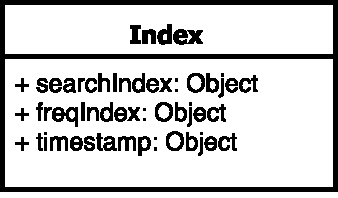
\includegraphics[width=0.3\textwidth]{IndexClassDiagramm}
    \caption{Index Klassendiagrmm}
    \label{fig:indexclassdiagramm}
    \end{figure}
    
\begin{listing}[H]
\inputminted[
frame=lines,
framesep=2mm,
baselinestretch=1.2,
linenos,
breaklines=true
]{js}{sourcecode/IndexService/freqIndex.ts}
\caption{Frequenz Index}
\label{freqindex}
\end{listing}
    
\subsection{Index-Initialisierung}


Die Berechnung des Index ist eine der prozessorintensiven Aufgaben, sie ist Zeit- und Ressourcen-intensiv. Dies insbesondere aufgrund der vielen Lese-Zugriffe. Darum wird der Index wann immer möglich zwischengespeichert, sodass eine erneute Berechnung erspart bleibt. Sie bildet die Grundlage für die zentralen Funktionen (\gls{Keyword}-Ex\-trak\-tion und Suche) des Prototyps. Um den Index zu initialisieren werden drei verschiedenen Szenarien unterschieden, der Ausgang diese Szenarien ist dabei immer der \gls{ikc-core}:
\begin{itemize}
    \item \textbf{Index Berechnen}: Es wurde noch keine Index berechnet, daher muss er von Grund auf neue berechnet werden.
    \item \textbf{Index Einlesen}: Der Index wurde bereits berechnet, jedoch noch nicht eingelesenen und bereit zu Verwendung. Dazu werden müssen die nötigen Daten abgefragt und eingelesen werden.
    \item \textbf{Index Bereit}: Der \texttt{IndexService} hat den Index bereits eingelesen und ist bereit zu Verwendung.
\end{itemize}
Folgend werden die verschiedenen Szenarien weitererläutert

\subsubsection{Index Berechnung}
\autoref{fig:seqindexalreadybuilt} zeigt den aufwändigen Ablauf der Index Berechnung. 
\begin{itemize}
    \item \texttt{requestIndex}: Der \gls{ikc-core} möchte Zugriff auf den Index. Dafür tätigt er eine Anfrage beim \texttt{IndexService}. Da der Index weder geladen noch je berechnet wurde, muss dieser neu berechnet werden.
    \item \texttt{dataRequest}: Dafür müssen zunächst alle Dokumente eingelesen werden. Dafür muss eine Anfrage an den \texttt{DataService} gemacht werden.
    \item \texttt{dataResponse}: Diese wird mit den geforderten Daten beantwortet.
    \item \texttt{parseData}: Die Daten werden geparst damit sie weiterverarbeitet werden können.
    \item \texttt{buildIndex}: Nun wird jedes einzelne Dokument, dem Index hinzugefügt. \autoref{calcindex} zeigt die verschiedenen Schritte, welche dabei ausgeführt werden:
    \begin{enumerate}
        \item Das entsprechende Dokument wird dem \texttt{searchIndex} mithilfe der Methode \texttt{addDoc} hinzugefügt. Pro Dokument werden die drei Felder \texttt{body} (Inhalt), \texttt{title} (Title) und \texttt{length} (Anzahl Wörter) verwendet. Neben dem Dokument Objekt muss der \texttt{addDoc} auch noch eine eindeutige Identifikation mitgegeben werden, hier \texttt{doc.id}. Die Anzahl Wörter wird später für die Berechnung der relevanten Dokumente für ein bestimmtes \gls{Keyword} verwendet. (Zeile 2-6)
        \item Nun werden für das entsprechende Dokument die mög\-lich\-en \gls{Keyword}[s] extrahiert. Dazu werden gleichen Berechnung verwendet wie in \autoref{listing:}, \autoref{generatekeywords} und \autoref{filter}. (Zeile 8)
        \item Nun werden zum Abschluss die \gls{Keyword}[s], nach dem beschriebenen Schema (\autoref{indexstructure}, dem Frequenz Index hinzugefügt. (Zeile 10-21)
    \end{enumerate}
    \item \texttt{saveIndex}: Sobald der Index berechnet wurde, wird er im \texttt{In\-dex\-Store} gespeichert.
    \item \texttt{indexReady}: Dem \gls{ikc-core} wird gemeldet, dass der Index bereit ist.
\end{itemize}

    \begin{figure}[H]
    \centering
    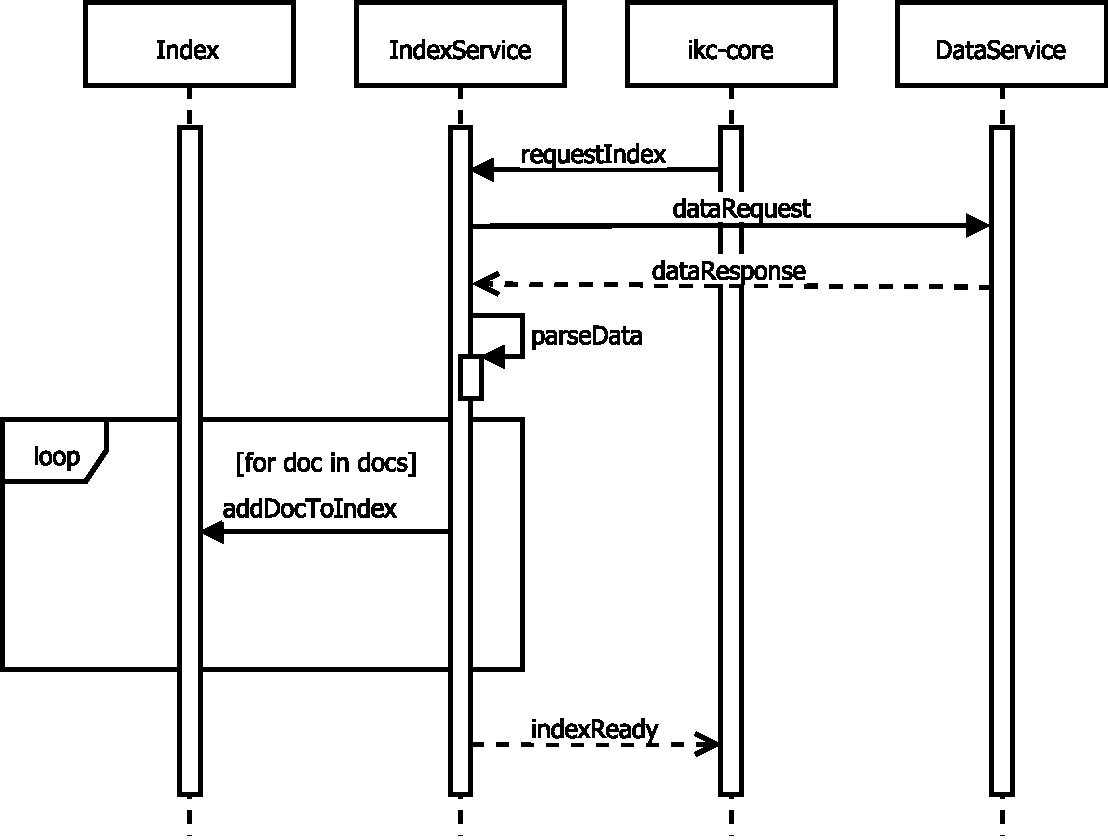
\includegraphics[width=1\textwidth]{SeqIndexLoad}
    \caption{Ablauf: Index-Berechnung}
    \label{fig:seqindexload}
    \end{figure}


\begin{listing}[H]
\inputminted[
frame=lines,
framesep=2mm,
baselinestretch=1.2,
linenos,
breaklines=true
]{js}{sourcecode/IndexService/calcIndex.ts}
\caption{Index Berechnen}
\label{calcindex}
\end{listing}
    
    
\subsubsection{Index Einlesen}

Falls ein Index bereits berechnet und persistiert wurde, muss er nur noch eingelesen werden. Diesen Ablauf wird in der \autoref{fig:seqindexalreadybuilt} erläutert. 
\begin{itemize}
    \item \texttt{requestIndex}: Der \gls{ikc-core} möchte Zugriff auf den Index. Dafür tätigt er eine Anfrage beim \texttt{IndexService}. Der \texttt{IndexService} hat den Index nicht geladen, er startet also die Berechnung.
    \item \texttt{dataRequest}: Nun muss das serialisierte Index-Objekt geladen werden. Dafür muss eine Anfrage an den \texttt{DataService} gemacht werden.
    \item \texttt{dataResponse}: Diese wird mit den geforderten Daten beantwortet.
    \item Die Daten werden eingelesen (\texttt{parseData}) und anschliessend verarbeitet (\texttt{loadIndex}). Die verschiedenen Schritte werden in \autoref{parseindex} detailliert erläutert.
    \begin{enumerate}
        \item Die empfangenen Daten (\texttt{body}) müssen mithilfe der externen Bibliothek \gls{msgpack} decodiert werden um die beiden Buffer für den Volltext und Frequenz Index zu erhalten.
        \item Nun werden die beiden Buffer zuerst dekomprimiert mit Hilfe der Bibliothek \gls{lz4} und anschliessend durch decodiert. Die Decodierung generiert aus dem Buffer ein Objekt. (Zeile 3-4)
        \item Nun werden die Decodierten Objekte dem \texttt{Index} zugwiesen. Der Volltext Index muss zuerst noch durch die \texttt{load} Methode des \gls{elasticlunr} eingelesen werden. (Zeile 6-7)
    \end{enumerate}
    \item \texttt{indexReady}: Dem \gls{ikc-core} wird gemeldet, dass der Index bereit ist.
\end{itemize}

    \begin{figure}[H]
    \centering
    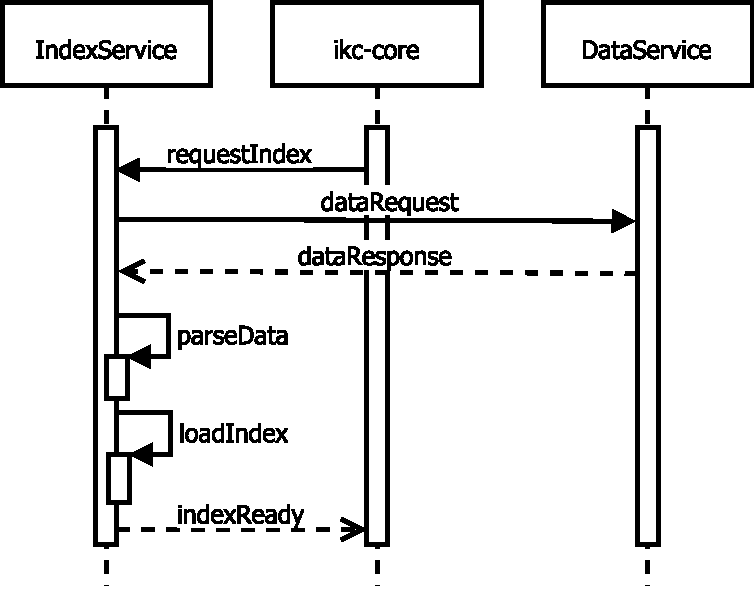
\includegraphics[width=1\textwidth]{SeqIndexLoadAlreadyBuilt}
    \caption{Ablauf: Index-Berechnung}
    \label{fig:seqindexalreadybuilt}
    \end{figure}
    
\begin{listing}[H]
\inputminted[
frame=lines,
framesep=2mm,
baselinestretch=1.2,
linenos,
breaklines=true
]{js}{sourcecode/IndexService/parseIndex.ts}
\caption{Index Objekt Laden}
\label{parseindex}
\end{listing}
    
    
\subsubsection{Index Bereit}
Die \autoref{fig:seqindexloadalreadydone} hingegen zeigt den Ablauf, falls der Index schon im \texttt{IndexService} geladen ist.

\begin{itemize}
    \item \texttt{requestIndex}: Der \gls{ikc-core} benötigt den Index. Dafür fragt er den \texttt{IndexService} an. Dieser hält den Index schon im Arbeitsspeicher bereit.
    \item \texttt{indexReady}: Somit kann er diesen direkt zurückliefern.
\end{itemize}
    
    \begin{figure}[H]
    \centering
    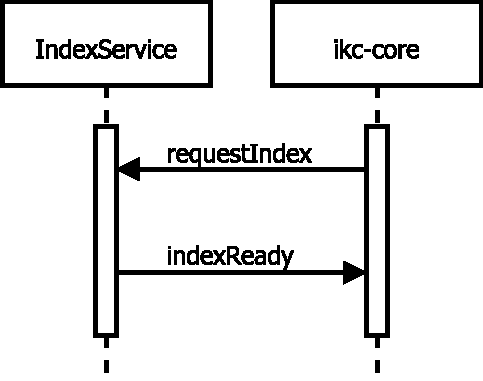
\includegraphics[width=0.5\textwidth]{SeqIndexLoadAlreadyDone}
    \caption{Ablauf: Index-Zugriff}
    \label{fig:seqindexloadalreadydone}
    \end{figure}
    
    
\subsection{Index Speichern}
Durch die Speicherung des Index werden die berechneten Daten gesichert und so eine aufwendige Neuberechnung verhindert. \autoref{fig:seqwriteindex} zeigt die einzelenen Schritte auf:
\begin{itemize}
    \item Das Speichern des Index wird durch den \gls{ikc-core} gelöst.
    \item Anschliessend wird der Index präpariert um diesen Persistieren zu können. Dazu sind die in \autoref{writeindex} beschriebenen Schritte notwendig:
    \begin{enumerate}
        \item Als erstes muss die \texttt{toJSON} Methode des \gls{elasticlunr} Objekts aufgerufen werden. Dadurch werden intern Funktionen für die serialisierung vorbereitet. (Zeile 2)
        \item Mit Hilfe der Bibliotheken \gls{msgpack} und \gls{lz4} werden die beiden Indices zuerst Codiert und anschliessend komprimiert. (Zeile 4-5))
        \item Zum Schluss werden beide resultierenden Buffer in einem Buffer zusammengefasst. (Zeile 7-11)
    \end{enumerate}
    \item Schlussendlich wird der präparierte Index an den \texttt{DataService} gesendet um diesen zu speichern. 
\end{itemize}

    \begin{figure}[H]
    \centering
    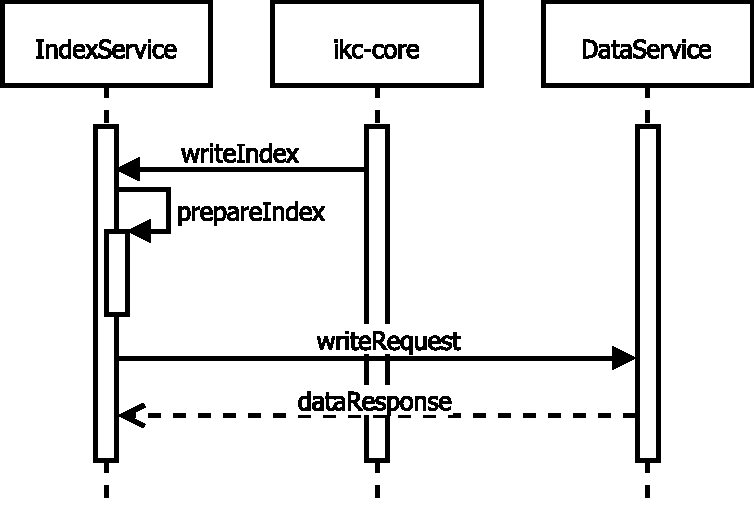
\includegraphics[width=0.5\textwidth]{SeqWriteIndex}
    \caption{Ablauf: Index Speichern}
    \label{fig:seqwriteindex}
    \end{figure}

\begin{listing}[H]
\inputminted[
frame=lines,
framesep=2mm,
baselinestretch=1.2,
linenos,
breaklines=true
]{js}{sourcecode/IndexService/writeIndex.ts}
\caption{Index Speichern}
\label{writeindex}
\end{listing}
    
\subsection{Keyword-Extraktion}
Die \gls{Keyword}-Extraktion ist eine der wichtigsten Funktion des Prototyps. Dabei werden die vorgestellten Abläufe und Code Ausschnitte aus dem \autoref{impalgo} verwendet. In der nachfolgenden \autoref{fig:seqkeywordextraction} wird der Ablauf genauer erläutert:
\begin{itemize}
    \item Initiiert wird die Extraktion von \gls{Keyword}[s] durch die \texttt{Key\-word\-Re\-qu\-est} Nachricht, welche der \gls{ikc-core} an den \texttt{IndexService} sendet. Anschliessend wir das entsprechende Dokument von dem \texttt{Da\-ta\-Ser\-vi\-ce} bezogen und für die verarbeitung Aufbereitet. 
    \item Innerhalb des \texttt{IndexService} werden die relevanten \gls{Keyword}[s] durch den \texttt{ExtractionService} berechnet und zurückgegeben.
    \item Anschliessend werden die \gls{Keyword}[s] innerhalb einer \texttt{Key\-word\-Re\-spon\-se} Nachricht an den \gls{ikc-core} gesendet.
\end{itemize}

    \begin{figure}[H]
    \centering
    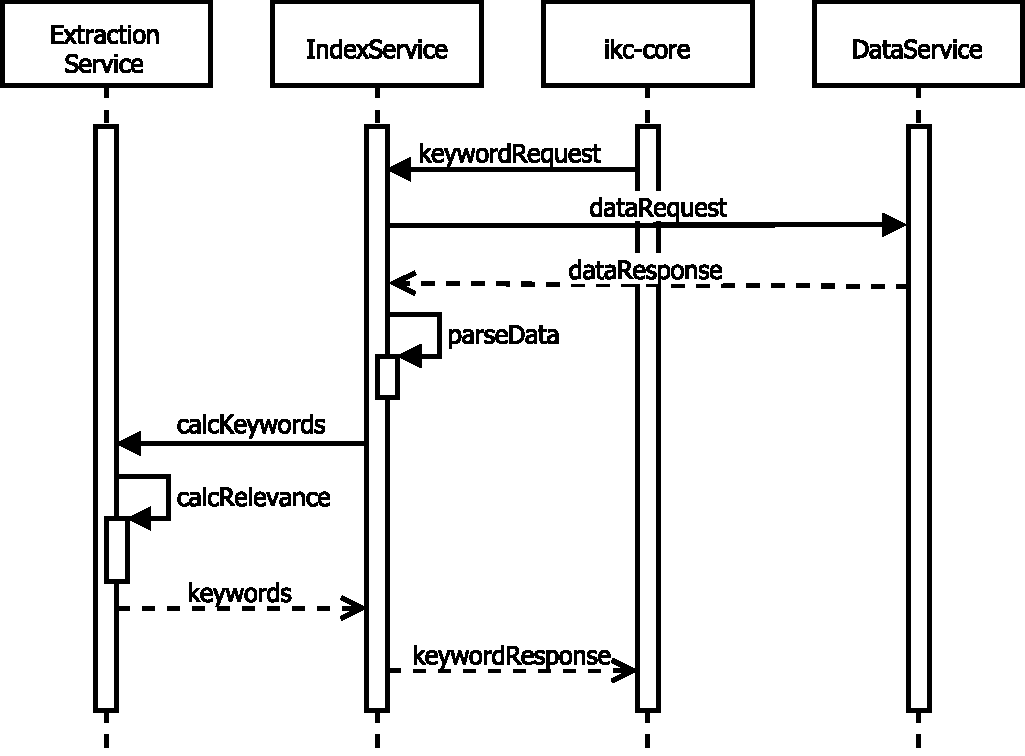
\includegraphics[width=1\textwidth]{SeqGetKeyword}
    \caption{Ablauf: \gls{Keyword} Extraktion}
    \label{fig:seqkeywordextraction}
    \end{figure}

\subsection{Dokument-Extraktion}

Neben der Extraktion von \gls{Keyword}[s] sollen pro \gls{Keyword} auch passende Dokumente extrahiert werden. Dieser Ablauf ist in der \autoref{fig:seqdocument} ersichtlich.

    \begin{figure}[H]
    \centering
    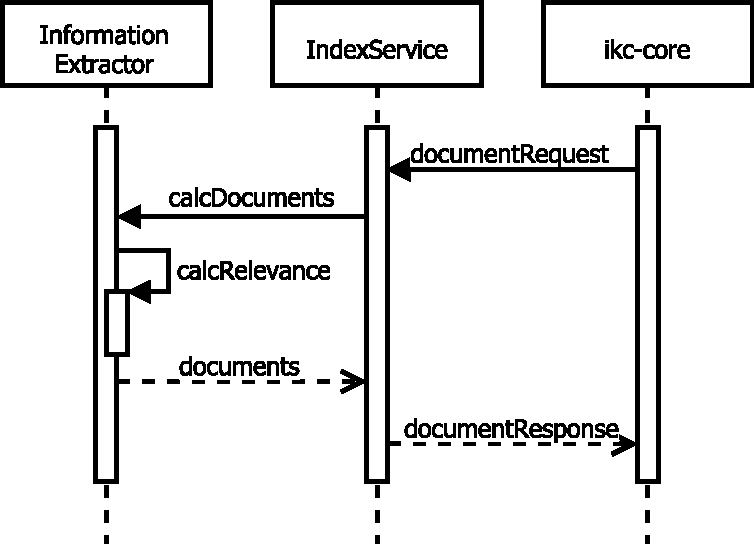
\includegraphics[width=0.8\textwidth]{SeqDocument}
    \caption{Ablauf: Dokument Extraktion}
    \label{fig:seqdocument}
    \end{figure}

\begin{itemize}
    \item der \gls{ikc-core} fordert durch eine \texttt{DocumentRequest} eine Liste von Dokumente für ein \gls{Keyword} an. 
    \item Anschliessend extrahiert der \texttt{InformationExtractor} eine Liste von passenden Dokumente und bewertet ihre Relevanz. 
    \item Innerhalb einer \texttt{DocumentResponse} Nachricht wird die resultierende Liste an den \gls{ikc-core} gesendet und die Anfrage somit beendet.
\end{itemize}

\subsection{Suche}

Um ganze Datenquellen zu durchsuchen wird eine Volltext Suche verwendet. Mit Hilfe der folgenden \autoref{fig:seqsearch}, wird der Ablauf der Suche aufgezeigt:
\begin{itemize}
    \item Innerhalb des \gls{ikc-core} wird eine Suchanfrage abgesetzt. Diese erreicht den \texttt{IndexService} eingebettet in einer \texttt{SearchRequest} Nachricht. 
    \item Intern arbeitet die \texttt{SearchService} die Suche ab und liefert die entsprechenden Resultate. \autoref{search} zeigt den Ablauf innerhalb des \texttt{SearchService}:
    \begin{enumerate}
        \item Um eine Suche durchführen zu können muss zuerst eine Konfiguration erstellt werden. Diese folgt der API Dokumentation von \gls{elasticlunr}. Sie wäre es möglich verschiedene Felder unterschiedlich zu gewichten. Auf diese Option wird jedoch verzichtet, legendlich die Option \texttt{bool} wird auf \texttt{AND} gesetzt. Damit müssen resultierende Dokumente alle Wörter der Suchanfrage enthalten. Eine andere Option wäre \texttt{OR} damit würden Dokumente resultieren die mindestens ein Wort der Suchanfrage enthält. (Zeile 2)
        \item Nun wird die eigentliche Suchanfrage ausgeführt, dazu wird die Methode \texttt{search} verwendet. Ihr wird der Suchterm (\texttt{term}) und die Konfiguration mitgegeben. Als Resultat wird eine Liste von Dokumentation Ids zusammen mit dem Score absteigend zurückgegeben. (Zeile 4)
        \item Durch die hohe Anzahl von zu erwartenden Dokumente, kann das Suchresultat sehr schnell Gross werden bei generellen Suchanfragen. Um das Resultat einschränken zu können, werden nur die 100 besten Resultate ausgewählt. Dies geschieht mithilfe der \texttt{slice} Methode der \texttt{Array} Klassen. Damit werden 100 Einträge innerhalb der Liste, ausgehend von Position null, ausgewählt. Fall weniger als 100 Einträge vorhanden sind, werden diese zurückgegeben. (Zeile 6)
        \item Anschliessend werden die Resultate in eine Liste von verwendbarer Information umgewandelt. Dazu wird für jedes Resultat, das entsprechende Dokument abgefragt (Zeile 10) und anschliessend dessen Id und Titel zurückgegeben. (Zeile 8-15)
    \end{enumerate}
    \item Die Resultate werden anschliessend in einer \texttt{SearchResponse} Nachricht eingebettet an den \gls{ikc-core} gesendet.
\end{itemize}

    \begin{figure}[H]
    \centering
    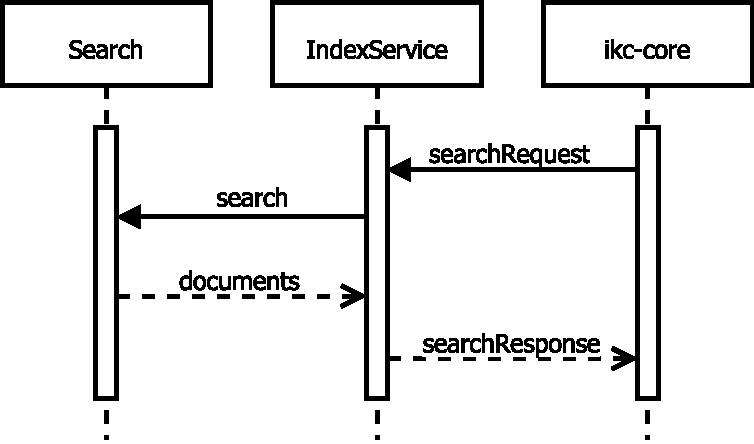
\includegraphics[width=0.7\textwidth]{SeqSearch}
    \caption{Ablauf: Suche}
    \label{fig:seqsearch}
    \end{figure}

\begin{listing}[H]
\inputminted[
frame=lines,
framesep=2mm,
baselinestretch=1.2,
linenos,
breaklines=true
]{js}{sourcecode/IndexService/search.ts}
\caption{Suche}
\label{search}
\end{listing}

\section{DataService}

Der \texttt{DataService} versorgt den \gls{ikc-core} und den \texttt{IndexService} mit den essentiellen Daten. Diese beinhalten die Textquellen an sich aber auch die verschiedenen Indizes. Diese werden über \gls{SSH} per \gls{SFTP} von einer externen Datenquelle angefordert und anschliessend bereitgestellt. 

    \begin{figure}[H]
    \centering
    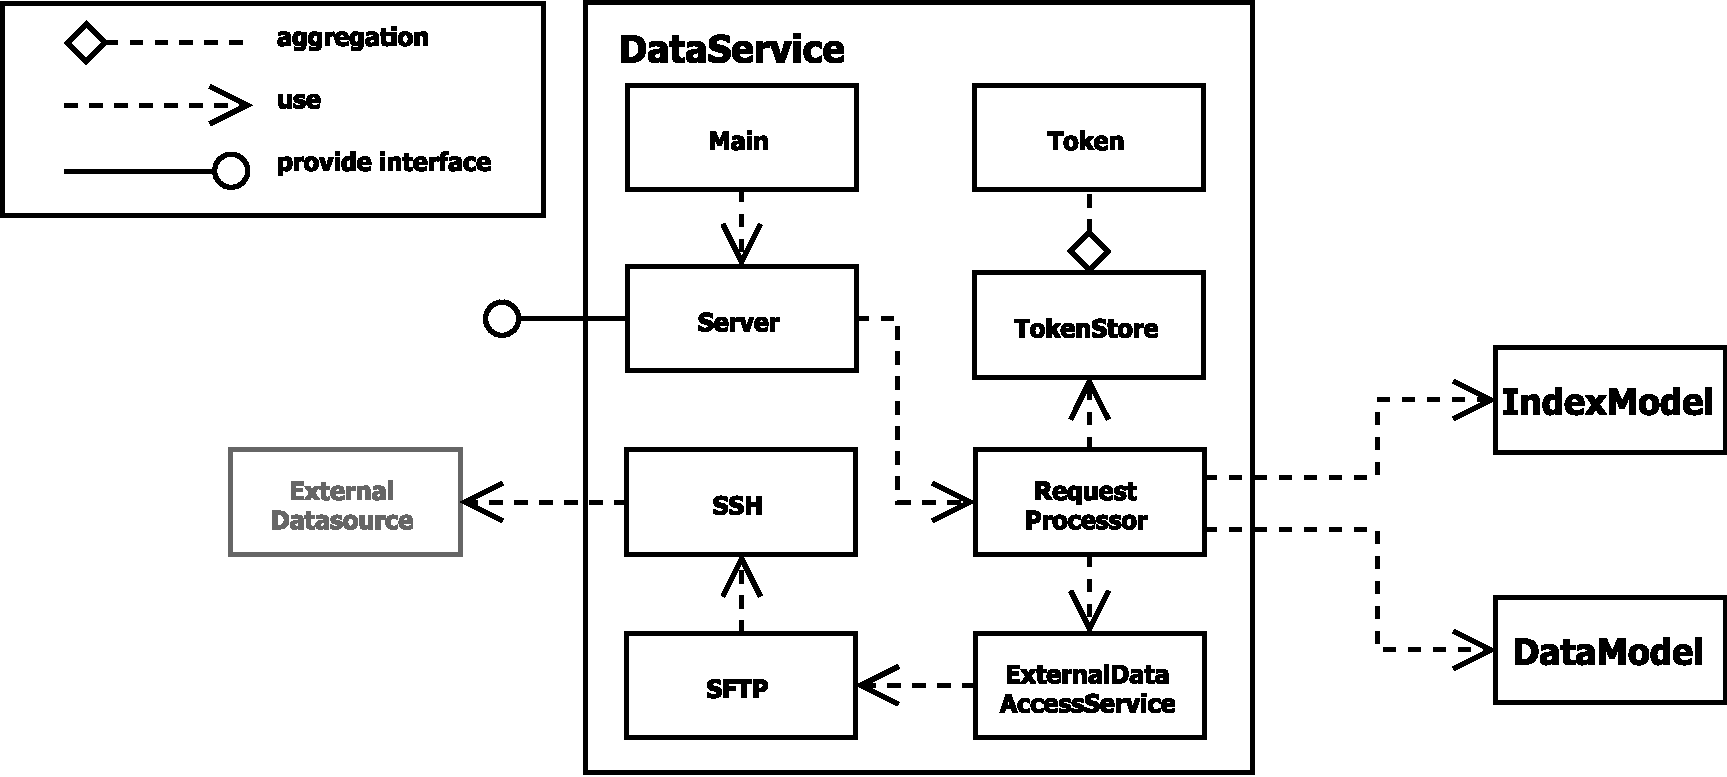
\includegraphics[width=1\textwidth]{DataServiceClassDiagram}
    \caption{DataService Klassendiagram}
    \label{fig:dataserviceClassDiagram}
    \end{figure}


\begin{itemize}
    \item \textbf{Server}: Auch hier hat der \texttt{Server} wiederum die Aufgabe Anfragen entgegenzunehmen und zu beantworten.
    \item \textbf{DataService}: Der \texttt{DataService} ist die Hauptklasse. Hier ist die zentrale Applikationslogik enthalten, Anfragen werden weitergeleitet. Die Anbindungen an eine Datenquelle wird ebenfalls von hier ausgesteuert.
    \item \textbf{TokenStore}: Das Zugriffskonzept mittels \gls{Token}[s] benötigt eine Zwischenspeicherung der Freigabeberechtigungen. Dies findet hier statt. 
    \item \textbf{SFTPService}: Ein Beispiel für eine externe Datenquelle ist \gls{SFTP}. Da der Zugriff hierbei über \gls{SSH} zu erfolgen hat, fungiert diese Klasse hier als Adapter.
    \item \textbf{SSHService}: Hier findet der eigentliche Zugriff auf die externe Datenquelle statt. Die Kommunikation geschieht über einen \gls{SSH}-Tunnel.
\end{itemize}


\section{Kommunikation}

Die Kommunikation zwischen den verschiedenen Service und Komponenten ist ein kritischer Faktor für die generelle Performance des gesamten Systems. Einerseits werden sehr viele Dateien über das Ne\-tz\-we\-rk übermittelt, andererseits muss damit ge\-rech\-net werden, dass einzelne Dateien Dateigrössen von 200 Megabyte überschreiten.

\subsection{Identifizierte Probleme}
\begin{enumerate}
    \item \textbf{Umgang mit grossen Dateien:} Grosse Dateien können aufgrund Begrenzungen des Arbeitsspeichers und oder Begrenzung der Datentypen nicht ohne weitere Schritte verwendet werden. Eine Lösung dafür ist die Verwendung von \gls{Stream}[s] und \gls{Buffer}[s].
    \item \textbf{Parsen und Serialisieren:} Die Übersetzung von rohe Binärdaten in ein Objekt und umgekehrt, ist bei grossen Dateien ebenfalls nicht trivial. \texttt{JSON.parse} und {JSON:stringify} funktionieren nicht ohne weiteres.
\end{enumerate}

\texttt{socket.io}\footnote{\url{https://github.com/socketio/socket.io/}} ist eine viel versprechende Bibliothek. Sie ist in praktisch allen gängigen Programmiersprachen implementiert, darum gibt es auch zahlreiche Erweiterungen. Ebenfalls gibt es eine Erweiterung für die Verwendung von \gls{Stream}[s] namens \texttt{socket.io-stream}\footnote{\url{https://github.com/nkzawa/socket.io-stream}}.

Für die Serialisierung und das Parsen wird zusätzlich \texttt{msgpack}\footnote{\url{http://msgpack.org}} verwendet. Es arbeitet problemlos mit grossen Dateien.

Die \autoref{fig:kommunikation} zeigt die schlussendlich verwendeten Technologien im Überblick. Die Grundlage der Kommunikation zwischen \gls{ikc-core}, \texttt{DataService} und \texttt{IndexService} bildet \texttt{TCP/IP}. Darüber läuft das abhörsichere \texttt{HTTPS}-Protokoll. Im \texttt{JavaScript} wird die Bibliothek \texttt{socket.io} mit der oben erwähnten \gls{Stream}-Erweiterung verwendet. \texttt{msgpack} übersetzt die binären Rohdaten in Objekte und umgekehrt.



    \begin{figure}[H]
    \centering
    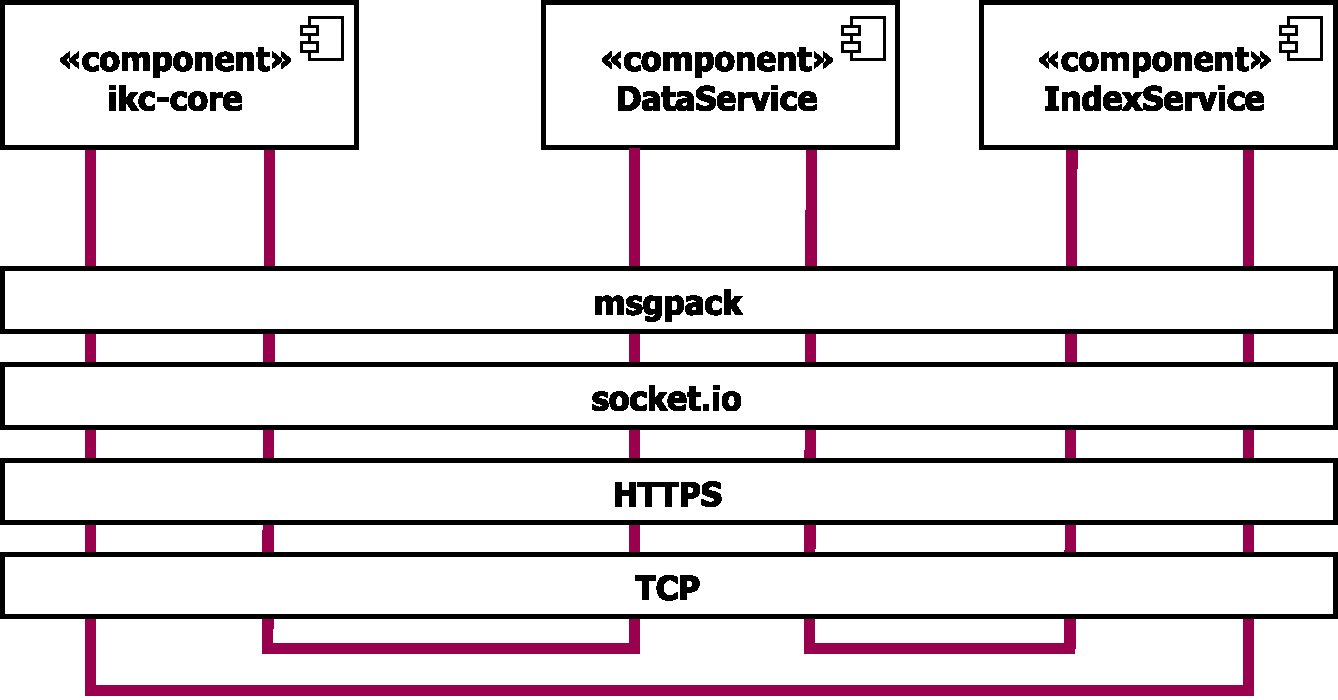
\includegraphics[width=1\textwidth]{ComponentDiagramm}
    \caption{Kommunikation}
    \label{fig:kommunikation}
    \end{figure}
    


\subsection{Protokoll}\label{section:protokoll}

Das Protokoll gibt an, in welchem Format die Daten übermittelt werden, sodass sie von beiden Seiten korrekt interpretiert werden. Es setzt also noch eine zusätzliche Ebene auf das obige Diagramm (\autoref{fig:kommunikation}) auf.


%    \begin{figure}[ht]
%    \centering
%    
\includegraphics[width=0.5\textwidth]{Protocol}
%    \caption{Protokoll Aufbau}
%    \label{fig:protocol}
%    \end{figure}

Die Kommunikation mit dem \texttt{IndexService} und dem \texttt{DataService} verläuft komplett eigenständig. Darum verwenden beide Services ein eigenes Protokoll. Für die Kommunikation mit einem Service muss das jeweilige Protkoll auch von der Gegenseite eingesetzt werden. Die Bedingung ist, dass alle übermittelnden Daten eine Instanz einer Klasse aus dem jeweiligen Protokoll sind.
    
%Diagramm Ablauf ala \url{http://www.hsg-kl.de/faecher/inf/netze/fehler2/index.php} 
%Diagramm Stack oder level evt. mit Diagramm kabel mit verschiedenen schichten oder standard protocol stack \url{https://www.google.ch/url?sa=i&rct=j&q=&esrc=s&source=images&cd=&ved=0ahUKEwjJ5uO57drTAhUGvRoKHZIbBE4QjhwIBQ&url=http%3A%2F%2Fgeti2p.net%2Fnl%2Fdocs%2Fprotocol&psig=AFQjCNEHKXFjqJgGFF7pzQhblQm2WwWp6w&ust=1494145920025872}

Grundsätzlich besteht jede Nachricht aus einem Objekt der abstrakten Klasse \texttt{Mes\-sa\-ge}. Es stammt vorzugsweise aus der \texttt{MessageFactory}, um die Erzeugung des Objektes zusätzlich zu entkoppeln. Eine \texttt{Mes\-sa\-ge} besteht immer aus 

\begin{itemize}
    \item \textbf{einer \texttt{UUID}},\\
    Diese identifiziert eine Nachricht eindeutig. Sie besteht aus einem zufällig generierten alphanumerischen Muster.
    \item \textbf{einem \texttt{MessageType}}\\
    Damit die Nachricht jederzeit und an allen dafür vorgesehen Orten richtig interpretiert werden kann, besitzt sie einen für den jeweiligen Zweck vorgesehenen Typ. Dieser gibt explizit an, wie die Nachricht aufgebaut ist und welchen Zweck sie hat.
    \item \textbf{und einem \texttt{Messagebody}}
    Dieser stellt der eigentliche Inhalt der Nachricht dar. Er enthält den für den jeweiligen Typ vorgesehenen Body.
\end{itemize}

Das Klassendiagram (\autoref{fig:messageClassDiagram}) zeigt den Aufbau der abstrakten Klasse \texttt{Message} noch etwas detaillierter auf. Wie man erkennen kann, handelt es sich beim \texttt{MessageBody} um ein \texttt{Interface}, beim \texttt{MessageType} um einen \texttt{Enumerator}. Der \texttt{MessageBody} kann somit jeweils eine für den Zweck passende Instanz halten. Eine abstrakte Klasse wird aus dem Grund eingesetzt, dass die \texttt{id} zwingend bei jeder Unterklasse gesetzt wird.

    \begin{figure}[H]
    \centering
    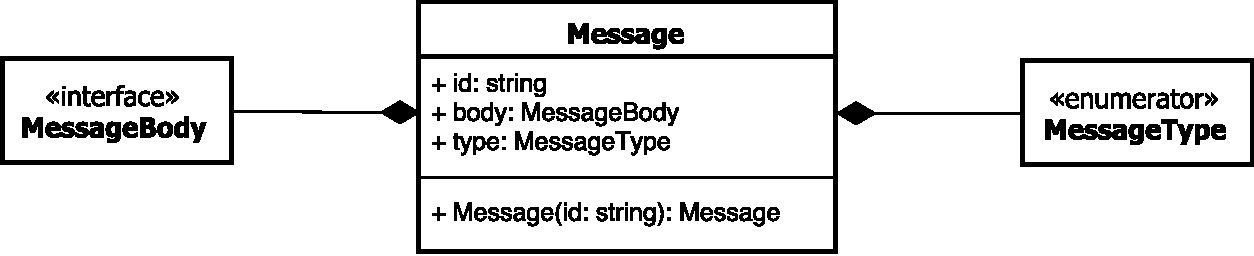
\includegraphics[width=1\textwidth]{MessageClassDiagram}
    \caption{Message Klassendiagram}
    \label{fig:messageClassDiagram}
    \end{figure}

\subsection{DataService-Protokoll}

\autoref{fig:dataclass} zeigt den Aufbau des \texttt{DataService}-Protokolls, dieses liegt im eigenen Paket \texttt{DataModel}. Dieses Protokoll wird im Prototyp für die Kommunikation zwischen \gls{ikc-core} und \texttt{DataService} beziehungsweise \texttt{IndexService} und \texttt{DataService} verwendet.

Im obigen Abschnitt (\autoref{section:protokoll}) wurde der Grundaufbau einer Nachricht aufgezeigt. Das \texttt{DataService}-Protokoll wird prinzipiell für den Datentransport eingesetzt. Das Protokoll gibt die dafür zu verwendenden Typen (\texttt{MessageTyp}) und Bodies (\texttt{MessageBody}) an. Die folgende Tabelle gibt einen Überblick über die verschiedenen Optionen. Zusätzlich zeigt das Ablaufdiagramm (\autoref{fig:seqdataprotocol}) einen vorstellbaren Beispielablauf mit den beteiligten Komponenten \gls{ikc-core} und \texttt{DataService}. Grundsätzlich folgt auf einen \texttt{Request} stets die entsprechende \texttt{Response}. Davon ausgenommen ist der Fehlerfall, wobei eine \texttt{ErrorResponse} zurückgeliefert wird.

\begin{longtable}{|p{4cm}| p{8cm}|}
  \hline
    \textbf{Bezeichnung} & \textbf{Beschreibung}\\\hline
    \texttt{TokenRequest} & Hierbei geht es um die Anfrage für eine Freigabe einer Datei oder eines Verzeichnisses. Für diesen Zweck gibt es das \texttt{Interface} \texttt{AccessSession} es enthält alle nötigen Zugangsdaten zur Verbindung mit einer externen Datenquelle. \newline
    
    Im Diagramm (\autoref{fig:seqdataprotocol}) ist die Klasse \texttt{SFTPAccessSession} enthalten. Diese regelt als Beispiel den Zugriff auf einen SFTP-Server.
    \\\hline
    \texttt{TokenResponse} &    
    Hat der \texttt{DataService} die Anfrage erhalten, schickt dieser bei Erfolg einen Token zurück. Dies geschieht in Form der \texttt{TokenResponse}. Diese enthält einen \gls{Token}. Dieser ist eine einmalige Zugriffsfreigabe für eine Datei oder einen Ordner von der jeweiligen Datenquelle.\newline
    
    
    Der \gls{Token} ist ein zufälliger generierter String, welcher auf dem \texttt{DataService} mit der jeweiligen \texttt{AccessSession} abgelegt ist.\\\hline
    \texttt{DataRequest} & Auf eine \texttt{TokenResponse} folgt ein \texttt{DataRequest}. Ist ein \gls{Token} auf dem \texttt{DataService} hinterlegt. Kann mit Hilfe dieses innerhalb eines \texttt{DataRequests} die jeweilige Datei oder das jeweilige Verzeichnis angefragt werden. \\\hline
    \texttt{DataResponse} & Die Antwort auf einen \texttt{DataRequest} ist im besten Fall eine \texttt{DataResponse}. Diese enthält den angefragten Dateiinhalt. \\\hline
    \texttt{ErrorResponse} & Schlägt bei einer der obigen Anfragen etwas fehl, wird eine \texttt{ErrorResponse} mit dem jeweiligen Fehler zurückgegeben. Fehlerursachen können von sehr unterschiedlicher Natur sein, beispielsweise sind Netzwerkprobleme oder falsche Zugangsdaten vorstellbar.\\\hline
        \caption{DataService: Message-Klassen}
    \label{dataservice-bodies}
\end{longtable}


    \begin{figure}[H]
    \centering
    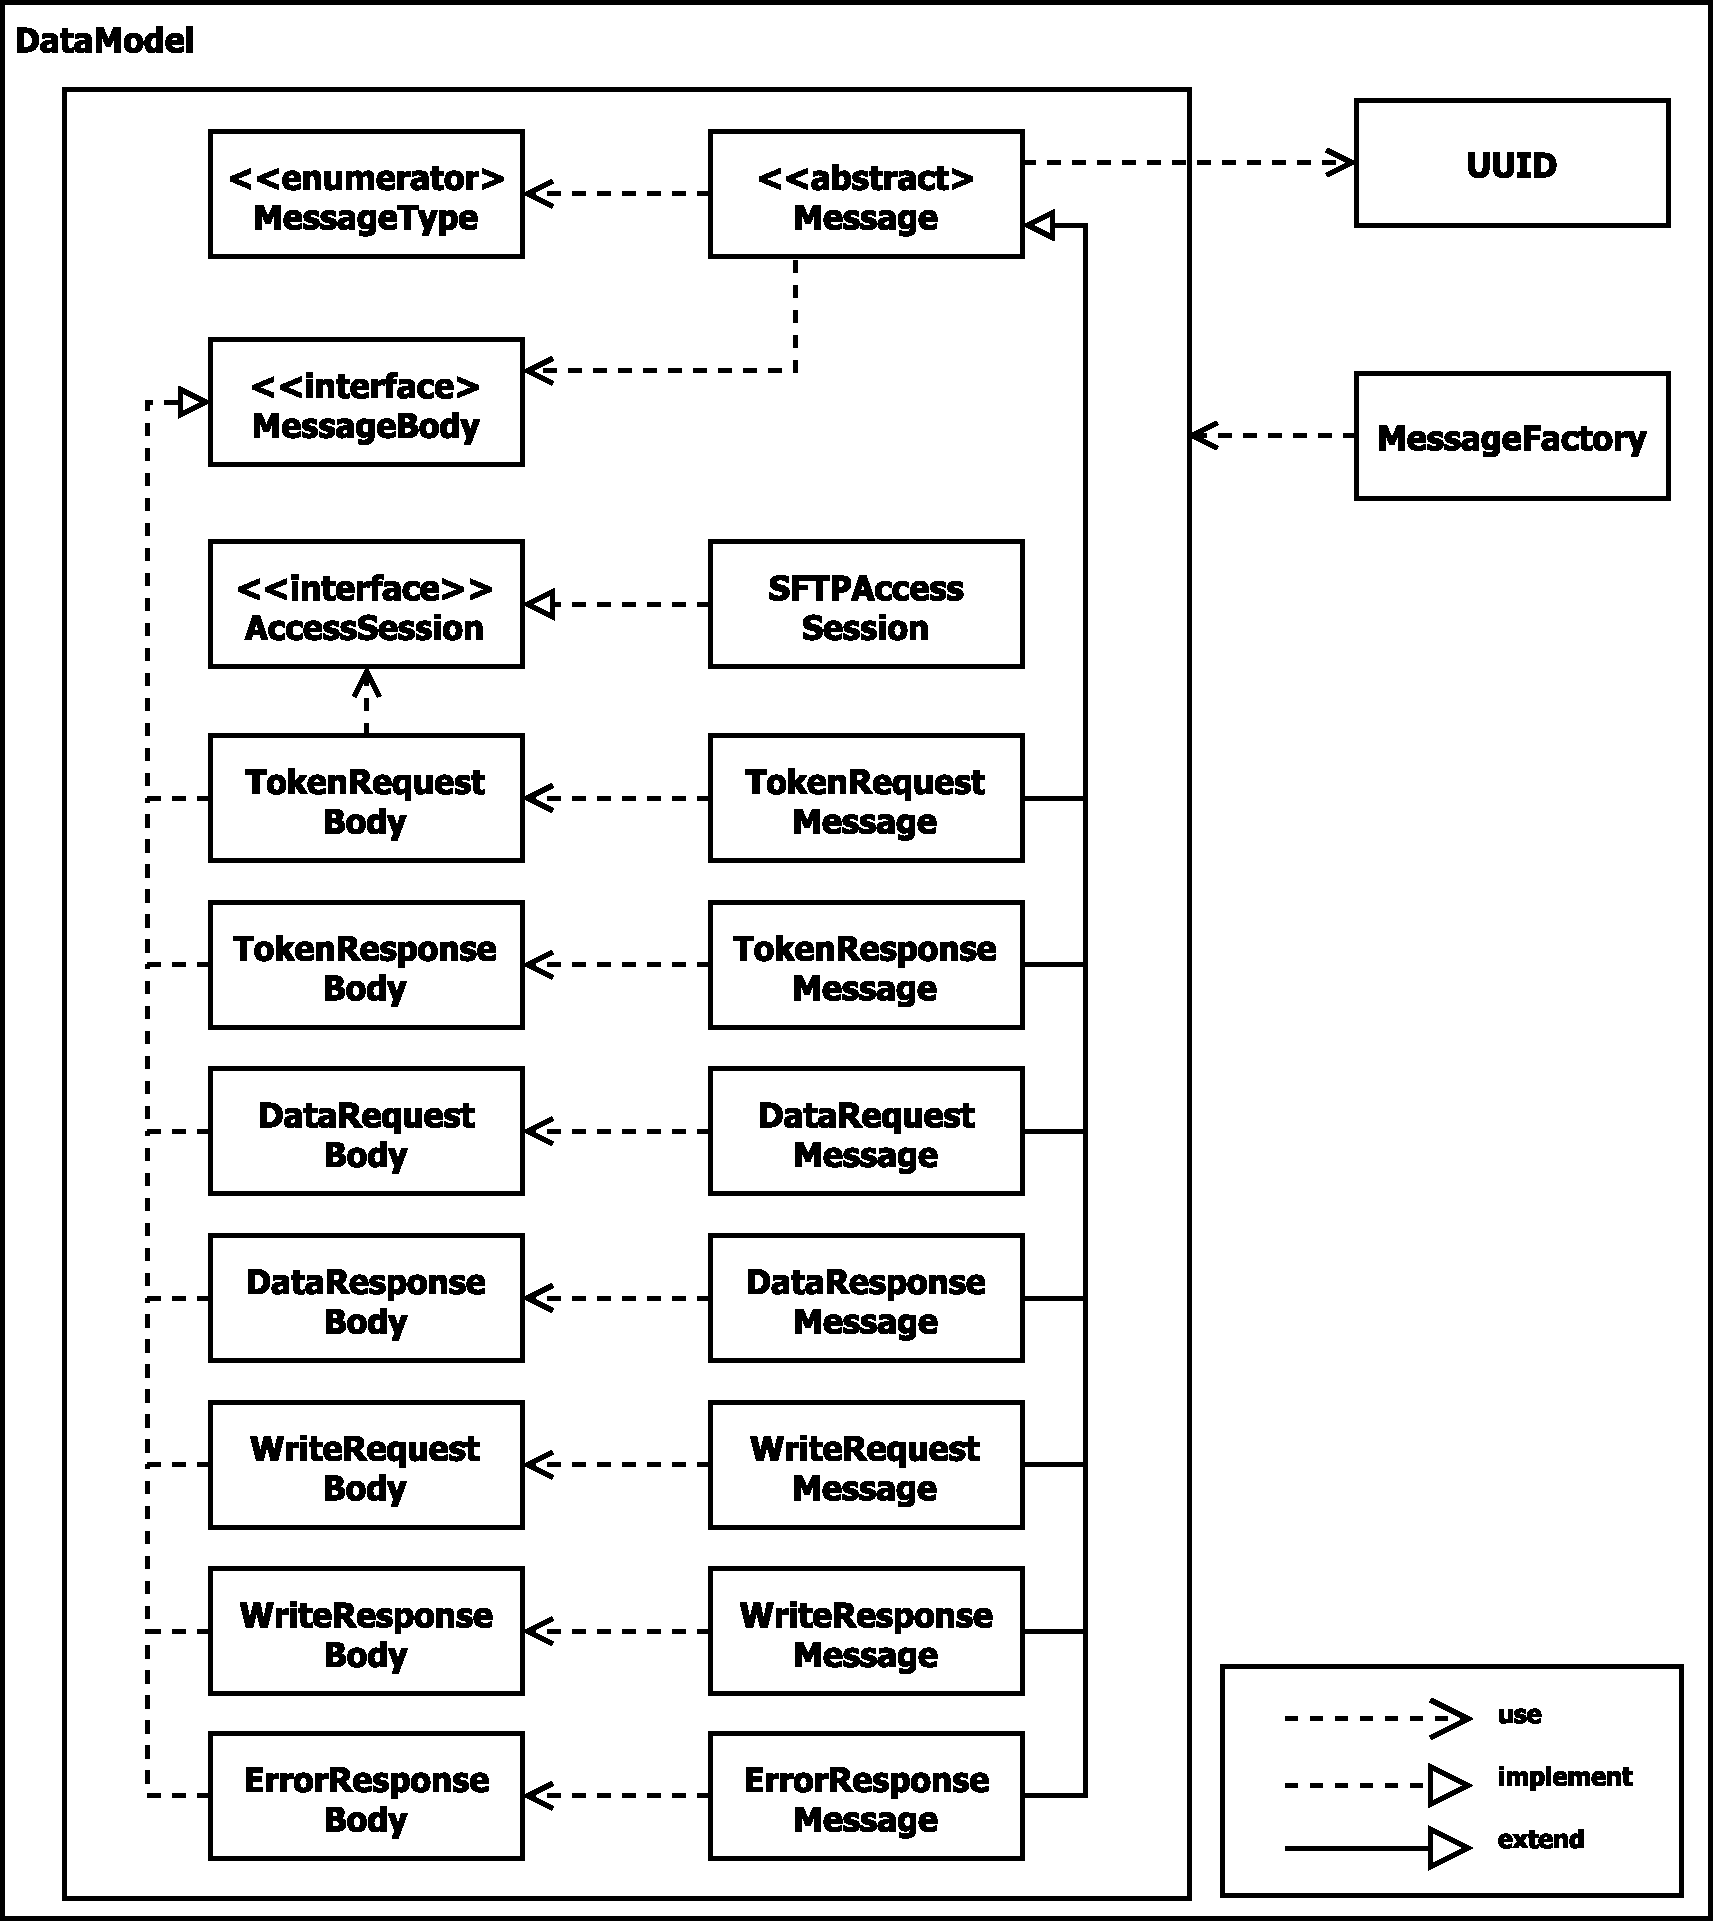
\includegraphics[width=0.9\textwidth]{DataModelClassDiagramm}
    \caption{Klassendiagramm DataService-Protokoll}
    \label{fig:dataclass}
    \end{figure}

    \begin{figure}[H]
    \centering
    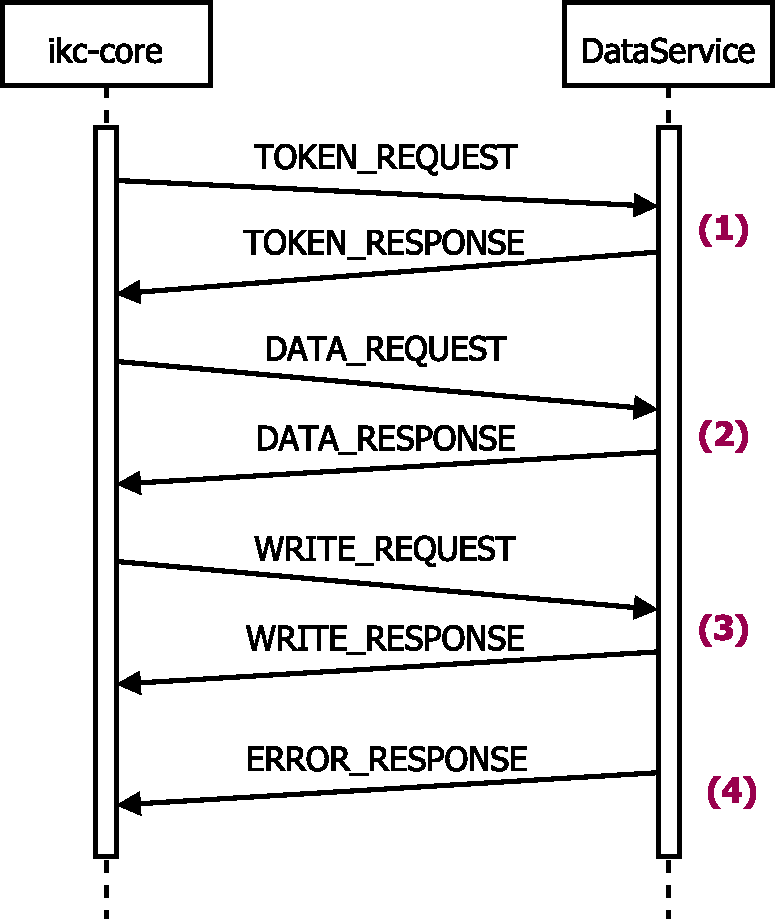
\includegraphics[width=0.5\textwidth]{DataModelSequence}
    \caption{Ablauf DataService-Protokoll}
    \label{fig:seqdataprotocol}
    \end{figure}


\subsection{IndexService-Protokoll}

Vom Aufbau her ähnlich wie das \texttt{DataService}-Protokoll sieht auch das \texttt{IndexService}-Protokoll aus (\autoref{fig:indexclass}). Wiederum ist die abstrakte Klasse \texttt{Message} die Grundlage. Allerdings unterscheiden sich die \texttt{Mes\-sa\-ge\-Typ\-es} und \texttt{MessageBodies}. Die Nachrichten haben hier den Zweck alle für die Volltextsuche und die Schlüs\-sel\-wort-\-Ex\-trak\-tion erforderlichen Daten zur Verfügung zu stellen.

    
    \begin{figure}[H]
    \centering
    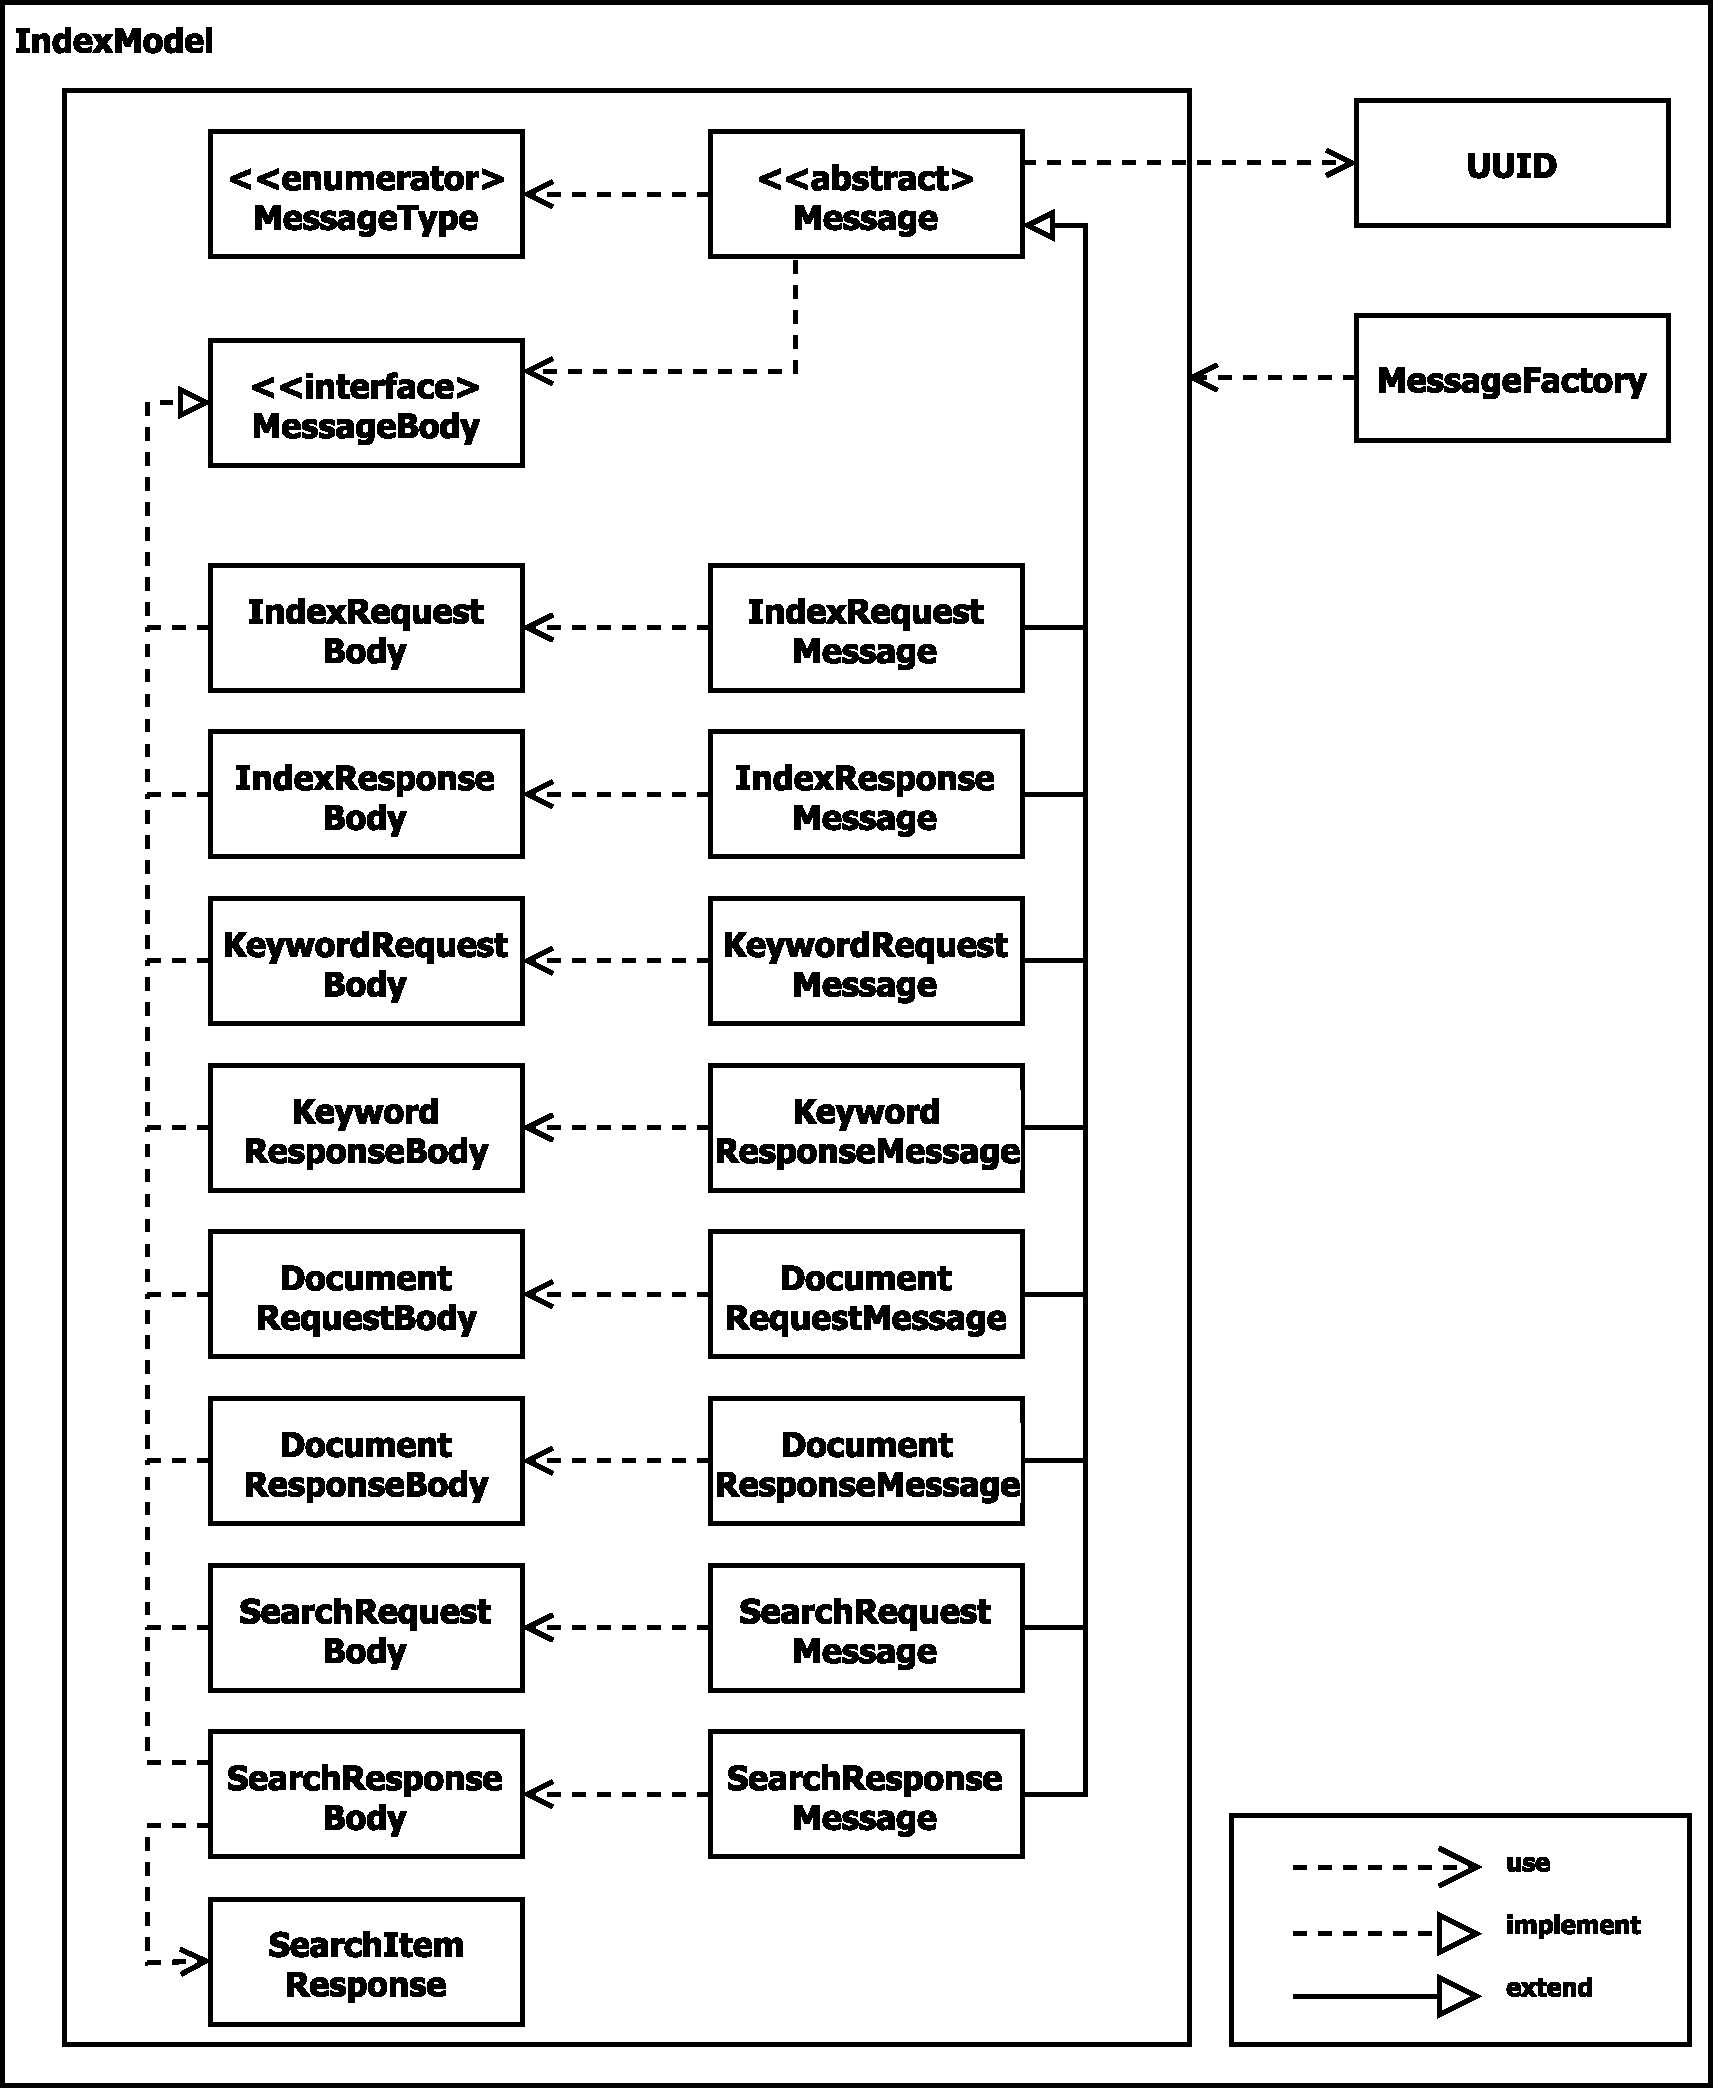
\includegraphics[width=1\textwidth]{IndexModelClassDiagramm}
    \caption{Klassendiagramm IndexService-Protokoll}
    \label{fig:indexclass}
    \end{figure}

Die Grundlage für die weiteren Vorgänge ist der Volltextindex. Dieser kann gelesen und persistiert werden. Ist diese Voraussetzung gegeben, können Schlüsselwörter für ein Dokument angefragt, zu einem Schlüsselwort passende Dokumente angefragt und Suche Resultate für einen bestimmten Begriff angefragt werden. Die Abläufe sind in der \autoref{fig:seqindexprotocol} ersichtlich. Die Vorgänge werden in folgender Tabelle genauer erläutert.

\begin{longtable}{|p{4cm}| p{8cm}|}
  \hline
    \textbf{Bezeichnung} & \textbf{Beschreibung}\\\hline
    \texttt{IndexRequest} & Der \texttt{IndexRequest} dient zum Anfragen des Volltextindex. Für diesen Vorgang wird zunächst der \gls{Token}, welcher zuvor beim \texttt{DataService} angefragt wurde, mitgeliefert. Zusätzlich dazu liegt der \texttt{Host} des anzufragenden \texttt{DataService} und die \texttt{indexId} ist die Identifikationsnummer des Index, falls dieser schon zuvor angefragt wurde.\\\hline
    \texttt{IndexResponse} & Nach der vorgängigen Anfrage für einen Index, folgt die Antwort in Form einer \texttt{IndexResponse}. Einziger Inhalt ist die \texttt{indexId} in Form eines Strings, welche den Index eindeutig identifizierbar macht.\\\hline
    \texttt{KeywordRequest} & Für die Schlüsselwort-Extraktion werden die Schlüsselwörter eines jeden Dokuments benötigt. Dafür gibt es den Vorgang \texttt{KeywordRequest}. Für die Verarbeitung werden ein \texttt{token} und ein \texttt{indexId} mitgeliefert. Der \texttt{token} hat seinen Ursprung wiederum im \texttt{DataService}. Er dient dazu den Volltext der jeweiligen Datei anzufragen. Die \texttt{indexId} ist wiederum dafür dazu da den gewünschten Index zu identifizieren.\\\hline
    \texttt{KeywordResponse} & Nach der obigen Anfrage folgt die Antwort in Form einer \texttt{KeywordResponse}. Diese beinhaltet ein Array von Strings, welches die extrahierten Schlüsselwörter des Dokumentes beinhaltet und die Identifikationsnummer des jeweiligen Dokumentes.\\\hline
    \texttt{DocumentRequest} & Sollen zu einem Schlüsselwort passende Dokumente angefragt werden, wird der \texttt{DocumentRequest} benutzt. Diese Anfrage beinhaltet das gesuchte Schlüsselwort und die Identifikationsnummer des jeweiligen Index.\\\hline
    \texttt{DocumentResponse} & Die Antwort beinhaltet wiederum das zuvor gesuchte Schlüsselwort und die Resultate als Array von Resultaten. Ein Resultat enthält den Titel, den Pfad, die Identifikationsnummer und den Inhalt des Dokumentes im Volltext.\\\hline
    \texttt{SearchRequest} & Eine weitere Funktionalität ist die Volltextsuche. Auch für diesen Zweck gibt es wiederum eine eigene Klasse. Um eine Suchanfrage abzusetzen, wird der Suchbegriff, eine Suchanfrage-Identifikationsnummer und wiederum eine \texttt{indexId} benötigt.\\\hline
    \texttt{SearchResponse} & Als Antwort auf eine Suchanfrage folgt ein Array von Suchresultaten. Ein Suchresultat enthält die Identifikationsnummer, den Pfad, den Titel und den Inhalt des gefundenen Dokuments.\\\hline
        \caption{IndexService: Message-Klassen}
    \label{indexservice-bodies}
\end{longtable}

    \begin{figure}[H]
    \centering
    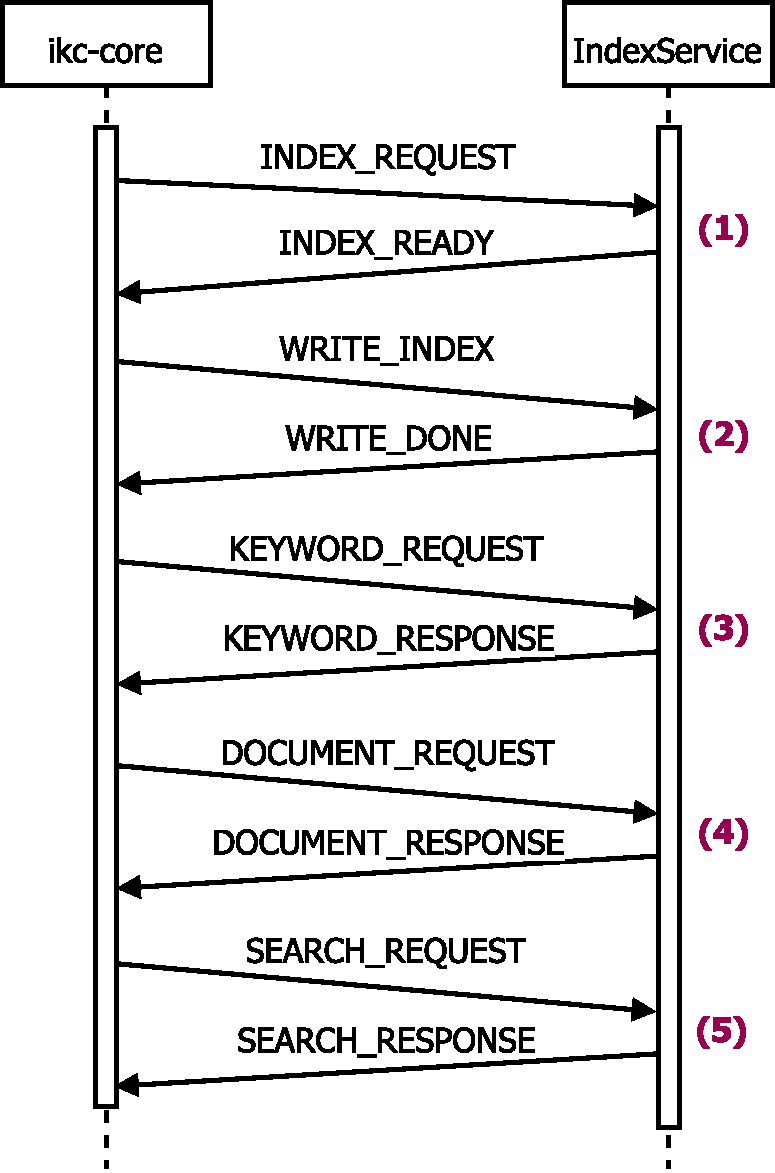
\includegraphics[width=0.5\textwidth]{IndexModelSequence}
    \caption{Ablauf IndexService-Protokoll}
    \label{fig:seqindexprotocol}
    \end{figure}

% -----------------------------------

\section{Daten}
    
\subsection{Quelle}

Als Datenquelle wird eine vom Auftraggeber zur Verfügung gestellte Sammlung von etwas mehr als 100'000 Wikipedia Artikeln verwendet. Diese enthalten qualitativ hochwertigen Informationen in Volltext und bilden die Grundlage für die Schlüsselwort-Extraktion und die Volltextsuche.

\subsection{Persistenz}

Im Gegensatz zum bestehenden Prototypen aus dem Forschungsprojekt \gls{IKC}, wird in dem hier vorliegenden als Datenquelle zusätzlich \gls{SFTP} ergänzt. Dies hat mitunter den Grund, wie in Absprache mit dem Auftraggeber festgelegt wurde, dass die erweiterte Anbindung an Cloud-Dienste, wie etwa Dropbox und Evernote, nicht der Kern dieser Bachelor-Arbeit ist. Der Fokus dieser Arbeit ist \textit{Information Retrieval} mittels \textit{Natural Language Processing} auf Basis von Schlüsselwort-Extraktion. Daher soll auch in diesem Bereich der Grossteil der zur Verfügung stehenden Zeit investiert werden. 

Aus diesem Grund werden die zu indexierenden Dateien, wie auch die Indizes und eventuelle Konfigurationsdateien auf einem \gls{SFTP}-Server gehalten.

\gls{SFTP} (SSH File Transfer Protocol) basiert auf \gls{SSH}, daher kann für die Authentifizierung direkt auch mit \gls{SSH}-Schlüssel gearbeitet werden. Für eine Verbindung mit einem \gls{SFTP}-Server sind folgende Daten notwendig:


\begin{longtable}{|p{4cm}| p{8cm}|}
  \hline
    \textbf{Bezeichnung} & \textbf{Beschreibung}\\\hline
    \texttt{host} & Dies entspricht dem Host-Namen oder der IP-Adresse des Servers, mit welchem verbunden werden soll.\\\hline
    \texttt{port} & Der Port gibt an, auf welchem Port der \gls{SFTP}-Server auf die Verbindung wartet. \gls{SSH} läuft standardmässig auf Port 22, dieser wird auch hier als Standardwert angenommen.\\\hline
    \texttt{user} & Dies ist der Benutzernamen für den Zugang zum Server. Dieser hat üblicherweise sein Verzeichnis auf dem jeweiligen Server.\\\hline
    \texttt{keyPath} & Wie oben schon erwähnt, wird für die Anmeldung kein Passwort, sondern direkt ein SSH-Private-Key verwendet. Der Dateipfad dazu wird hier angegeben.\\\hline
    \texttt{docDir} & Will der Benutzer nicht direkt mit seinem Stammverzeichnis arbeiten, hat er hier die Möglichkeit ein anderes Verzeichnis anzugeben. Die entsprechenden Berechtigungen dafür sind vorausgesetzt.\\\hline
        \caption{SFTP: Anmeldedaten}
    \label{sftp-anmeldung}
\end{longtable}


In \autoref{ssh-connection} sind die oben besprochenen Angaben zusätzlich in \gls{Typescript} ersichtlich. Das Objekt \texttt{config} enthält alle für die Verbindung nötigen Daten. Diese wurden in der Entwicklung des Prototyps so verwendet. Der Wert \texttt{docDir} zeigt hier auf das Verzeichnis des Benutzers \texttt{ikcdata}. Diese musste hier zusätzlich gesetzt werden, da der Benutzer Zugriff auf das Stammverzeichnis des Servers hat. Ohne eine zusätzliche Angabe würde der Service direkt auf dieses Verzeichnis zugreifen.


\begin{listing}[H]
\inputminted[
frame=lines,
framesep=2mm,
baselinestretch=1.2,
linenos,
breaklines=true
]{js}{sourcecode/dataservice/ssh-connection.ts}
\caption{SSH-Verbindung}
\label{ssh-connection}
\end{listing}

Auf Zeile 1 (\autoref{ssh-connection}) ist die für die Verbindung verwendete Bibliothek \texttt{ssh2}\footnote{\url{https://github.com/mscdex/ssh2}} zu sehen.


\begin{listing}[H]
\inputminted[
frame=lines,
framesep=2mm,
baselinestretch=1.2,
linenos,
breaklines=true,
]{js}{sourcecode/dataservice/ssh-sftp.ts}
\caption{SSH: SFTP-Client}
\label{ssh-sftp}
\end{listing}

%\begin{listing}[H]
%\inputminted[
%frame=lines,
%framesep=2mm,
%baselinestretch=1.2,
%linenos,
%breaklines=true,
%firstline=6, 
%lastline=33,
%highlightlines={7, 21-24}
%]{js}{sourcecode/dataservice/ssh-sftp.ts}
%\caption{SSH: SFTP-Client}
%\label{ssh-sftp}
%\end{listing}


Die Bibliothek liefert nach dem Aufbau der \gls{SSH}-Verbindung zum Server ein \gls{SFTP}\gls{Stream}-Objekt zurück (\autoref{ssh-sftp} Zeilen 21-24)\footnote{Dokumentation zu Client-Methoden \url{https://github.com/mscdex/ssh2}}. Dieser \gls{Stream} bietet die gewünschte Funktionalität zum Lesen und Schreiben von Verzeichnissen oder Dateien.\footnote{\url{https://github.com/mscdex/ssh2-streams/blob/master/SFTPStream.md}} Selbstverständlich kann die zugrundeliegende \gls{SSH} auch direkt weiterverwendet werden. Dies ermöglicht beispielsweise eine einfache Auswertung und schnellen Vergleich über externe Änderungen auf Datei-Ebene.


\subsection{Freigabe}
Für den Auftraggeber ist eine sichere Kommunikation und stetige Transparenz und Kontrolle über den Verbleib von benutzergenerierten Daten von hoher Wichtigkeit. Um diesen Anforderungen gerecht zu werden, wurde unter anderem ein Datenfreigabe-Konzept entwickelt. Dieses basiert auf \gls{Token}[s]. Die Vorgehensweise kann mittels der \autoref{fig:seqaccesssession} gut aufgezeigt werden.

\begin{itemize}
    \item \texttt{requestToken}: Ein generischer Kunde (\texttt{<<customer>>}) möchte eine Datei von der externen Datenquelle beziehen. Zunächst muss er dafür den \texttt{Da\-ta\-Ser\-vi\-ce} für einen Freigabe-\gls{Token} anfragen. Dabei müssen bei der Anfrage Informationen, wie die gesamte Zugriffsberechtigung (\textit{Host}, \textit{User}, \textit{SSH-PrivateKey}) und der Pfad der Datei mitgegeben werden. Die Zugriffsberechtigung muss eigenhändig vom Benutzer hinterlegt werden.
    
    \item \texttt{generateToken}: Der \texttt{DatService} verarbeitet die Anfrage und generiert mit den gegebenen Informationen ein \gls{Token}.
    
    \item \texttt{storeToken}: Dieser \gls{Token} wird im Hintergrund mit der zu\-ge\-höri\-gen Zugangsberechtigung und dem Dateipfad für spätere Verwendung im \texttt{TokenStore} hinterlegt.
    
    \item \texttt{token}: Nun wird der \gls{Token} als Antwort auf die Anfrage an den generischen Kunden zurückgeschickt.
    
    \item \texttt{dataRequest}: Prinzipiell kann nun jeder generische Kunde mit dem erhaltenen \gls{Token} eine Dateianfrage an den \texttt{DataService} tätigen. Dies kann er tun, ohne Kenntnis über die Zugangsberechtigung zu haben. Der \gls{Token} ist ausreichend. Aber Achtung: Die vergebenen \gls{Token}[s] sind nur für einen Zugriff gültig (one-way). Nach dem ersten Gebrauch werden diese, und auch die zugehörigen Zugriffsberechtigungen, verworfen!
    \texttt{getPathForToken}: Der \texttt{DataService} sucht im \texttt{TokenStore} die zum \gls{Token} zu\-ge\-hör\-igen Daten. Dazu zählen einerseits die Zugangsberechtigung zur Datenquelle und andererseits der Dateipfad.
    
    \item \texttt{path}: Diese Daten werden an den \texttt{DataService} retourniert.
    \item \texttt{read}: Nun kann der \texttt{DataService} die Daten von der externen Datenquelle anfordern.
    \item \texttt{data}: Auf die Anfrage folgt eine Antwort, welche die ge\-wünsch\-ten Daten zurückliefert.
    \item \texttt{dataResponse}: Diese werden an den Kunden zurückgegeben.

\end{itemize}


%ablaufdiagramm Einwegtoken Entkopplung

    \begin{figure}[H]
    \centering
    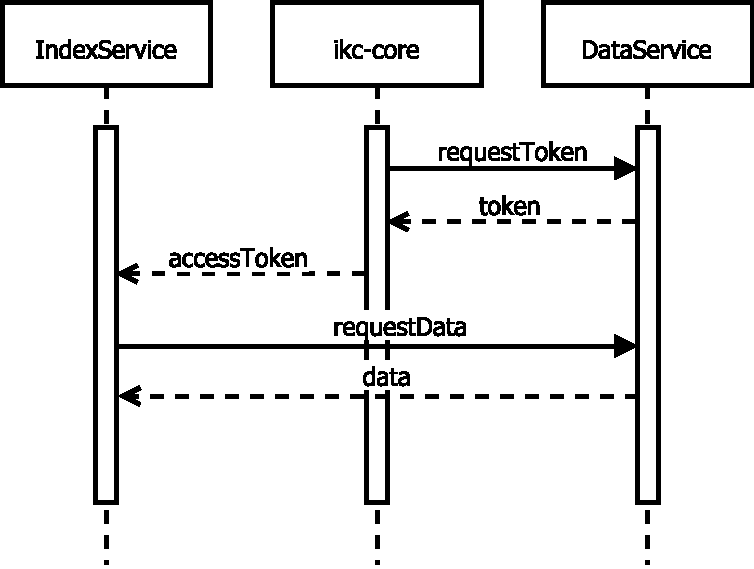
\includegraphics[width=0.8\textwidth]{SeqAccess}
    \caption{Ablauf: Datenfreigabe}
    \label{fig:seqaccesssession}
    \end{figure}


\section{MessageManager}\label{message-manager}

Sowohl im \texttt{Dataservice} als auch im \texttt{IndexService} wird ein \texttt{MessageManager} verwendet um eingehende Nachrichten zu verarbeiten. Ein besonderes Augenmerk wurde dabei auf die Entkopplung der Verarbeitung und der Handhabung der einzelnen Nachrichten. Dazu werden \textit{Traits} verwendet. Mit welchen zur Laufzeit das Verhalten einer Klasse angepasst werden können. Dies geschieht durch das Ersetzten des Verhalten einer Funktion durch jenes des \textit{Traits}. \autoref{fig:mixin} zeigt die Verwendung von \textit{Traits} innerhalb des \texttt{MessageMangers}.

\begin{itemize}
    \item Die beiden Interface \texttt{Mapper} und \texttt{Processor} definieren die beiden Methoden \texttt{send} und \texttt{process}.
    \item Innerhalb des \textit{Trait} \texttt{Processor} wird die Abarbeitung der jeweiligen Nachricht implementiert. Dies geschieht durch die Implementation der \texttt{process} Methode des Interface \texttt{Processor}. Dazu wird pro Nachricht ein seperate \texttt{Trait} Klasse erstellt (z.b. \texttt{DataRequestProcessor} \autoref{data-request-processor}).
    \item Die Abbildung des Resultates auf eine Antwort-Nachricht wird durch einen jeweiligen \textit{Mapper} (z.b. \texttt{DataResponseMapper} \autoref{data-response-mapper}) durchgeführt. Dafür wird die Methode \texttt{map} implementiert, welche durch das Interface \texttt{Mapper} definiert wird.    
    \item Als Abstraktion einer eingehenden Nachricht dient die Klasse \textit{Request} (\autoref{message-manager}). Sie enthält die eingegangene Nachricht (\texttt{message}, Zeile 2) und ein \texttt{callback} (Zeile 3) um eine Antwort Nachricht zurückzugeben. Weiter ist die Methode \texttt{run} (Zeile 7-17) definiert, welche die beiden Methoden \texttt{process} (Zeile 8) und \texttt{map} (Zeile 9) ausführt und die resultierende Antwort-Nachricht zurück gibt (Zeile 10).
    \item Innerhalb des \texttt{MessageManager} wird schlussendlich die \texttt{Request} Klasse je nach Situation angepasst. Bevor die eignende Nachricht mittels der \texttt{run} Methode (Zeile 3) abgearbeitet werden kann, muss das entsprechendes Objekt generiert werden. Dazu wird die Methode \texttt{mixIn} (Zeile 5-12) verwendet, welche je nach Art der Nachricht (Zeile 7) die jeweiligen \textit{Traits} (Zeile 8) zuordnet und ein Objekt der \texttt{Request} Klasse instantiiert (Zeile 9). Dabei wird die Methode \texttt{applyMixins} (Zeile 14-20) verwendet, welche die beiden Methoden \texttt{process} und \texttt{map} mit den entsprechenden \textit{Traits} überschreibt (Zeile 17).
\end{itemize}

    \begin{figure}[H]
    \centering
    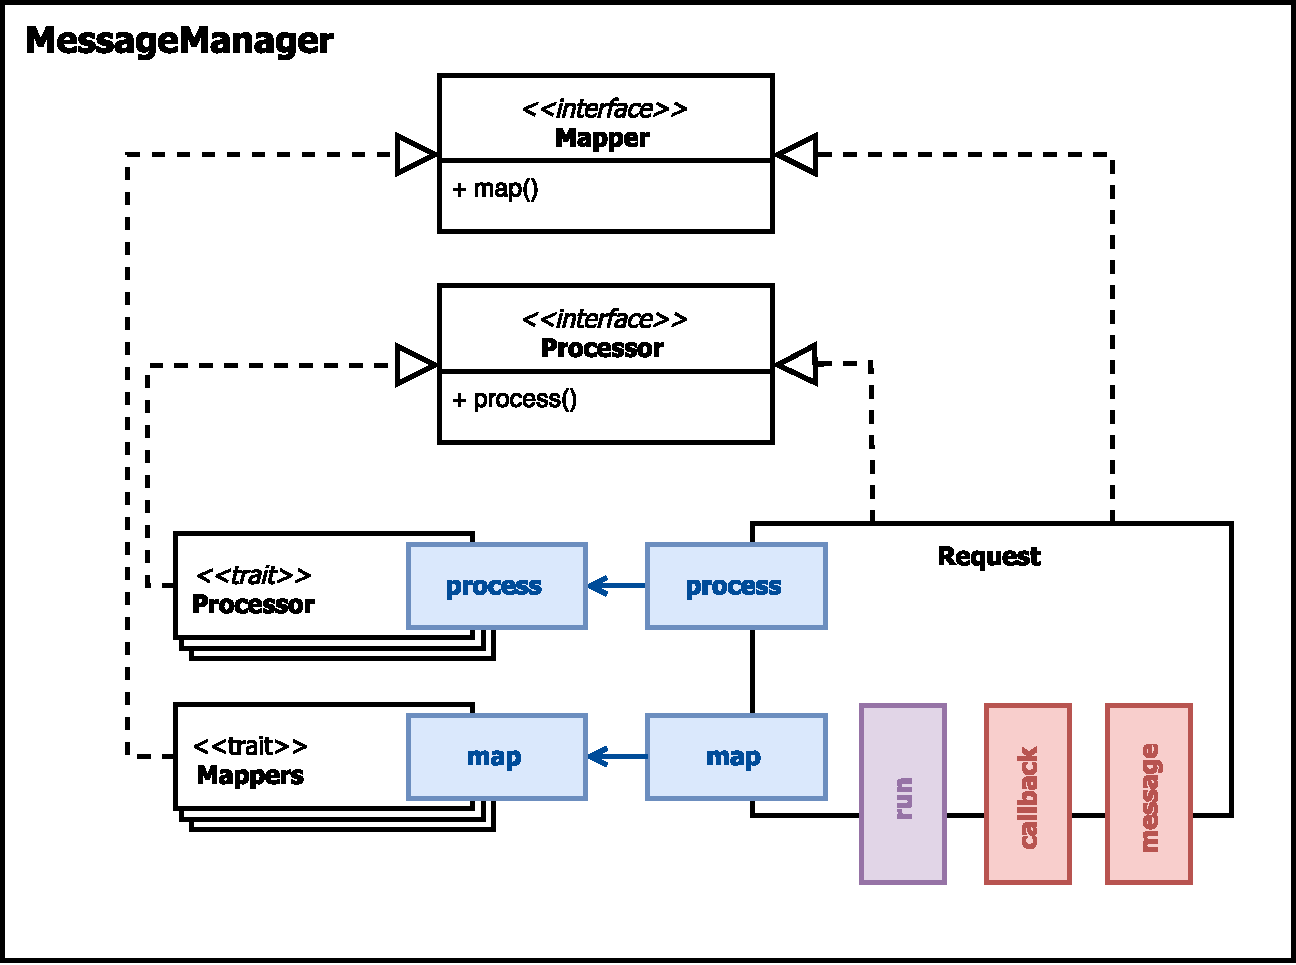
\includegraphics[width=0.8\textwidth]{Mixin}
    \caption{Funktionsweise MessageManager}
    \label{fig:mixin}
    \end{figure}
    
\begin{listing}[H]
\inputminted[
frame=lines,
framesep=2mm,
baselinestretch=1.2,
linenos,
breaklines=true
]{js}{sourcecode/DataRequestProcessor.ts}
\caption{DataRequestProcessor Implementation}
\label{data-request-processor}
\end{listing}

\begin{listing}[H]
\inputminted[
frame=lines,
framesep=2mm,
baselinestretch=1.2,
linenos,
breaklines=true
]{js}{sourcecode/DataResponseMapper.ts}
\caption{DataResponseMapper Implementation}
\label{data-response-mapper}
\end{listing}
    
\begin{listing}[H]
\inputminted[
frame=lines,
framesep=2mm,
baselinestretch=1.2,
linenos,
breaklines=true
]{js}{sourcecode/Request.ts}
\caption{Request Klasse}
\label{request-class}
\end{listing}


\begin{listing}[H]
\inputminted[
frame=lines,
framesep=2mm,
baselinestretch=1.2,
linenos,
breaklines=true
]{js}{sourcecode/MessageManager.ts}
\caption{Message Manager}
\label{message-manager}
\end{listing}

\section{Integration des Prototypen}

Der Prototyp soll sich möglichst Nahtlos in den \gls{ikc-core} integrieren. Um dies zu erreichen sollen in keiner Situation Funktionen des \gls{ikc-core} blockiert werden durch den Prototyp. 

So werden Suchresultate des Index innerhalb der bestehenden Suche integriert und bei Bedarf aktualisiert. Die verschiedenen Resultate der verschiedenen Quellen sollen in Echtzeit nach ihrem Eintreffen dargestellt werden. Somit wird sich die Liste mit Resultate trotz gleichem Suchbegriff über die Zeit verändern, da weitere Resultate von entfernten Quellen eintreffen. 

Weiter sollen extrahierte \gls{Keyword}[s] klar getrennt von den bestehenden Properties des Nodes als \textit{Chips} oberhalb des Titel dargestellt werden. Sowohl ein Dokument mit entsprechenden \gls{Keyword}[s] als auch eine \gls{Keyword} mit den verknüpften Dokumenten werden als Node dargestellt. \autoref{fig:bda_ui} zeigt einen Entwurf dieser Integration. 

    \begin{figure}[H]
    \centering
    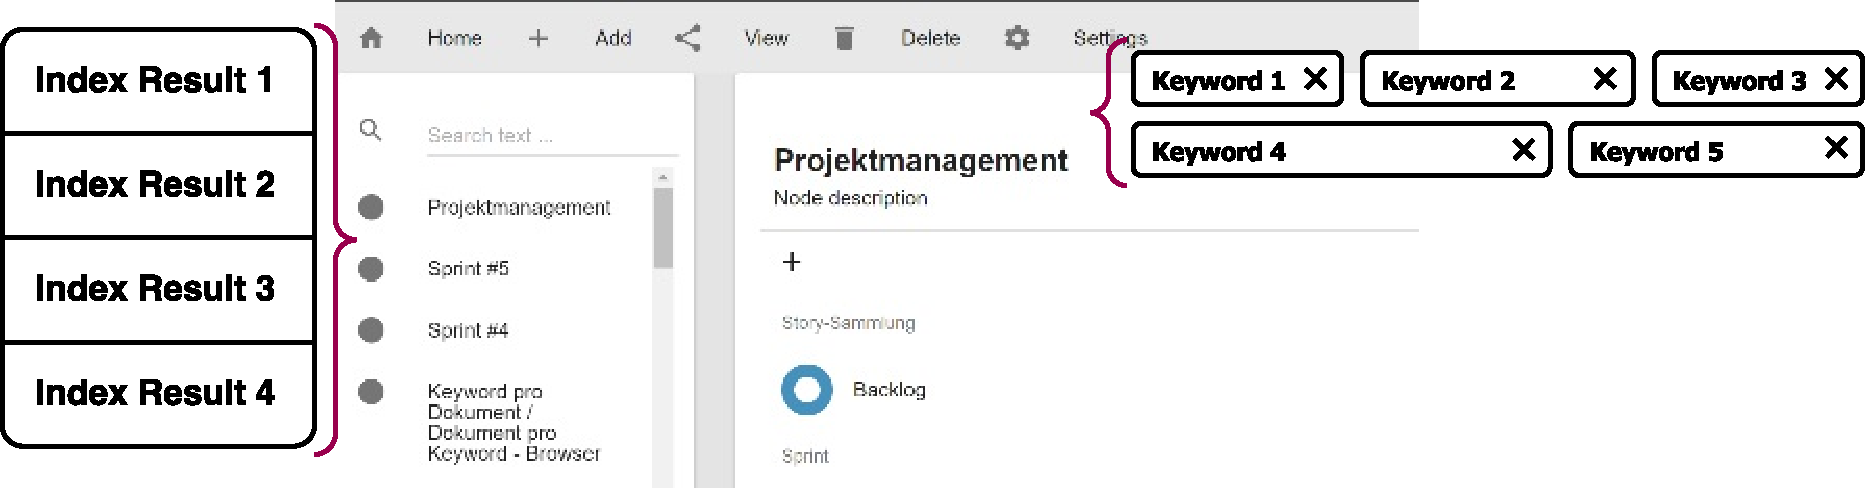
\includegraphics[width=1\textwidth]{BDA_UI}
    \caption{Entwurf Intgeration Benutzeroberfläche}
    \label{fig:bda_ui}
    \end{figure}

Um die Schnittstellen des Prototyps ideal zu verwenden und die obigen Oberflächenanpassungen umzusetzten, sind Anpassungen bzw. Erweiterungen in der Software Struktur des \gls{ikc-core} nötig. Das Klassendiagramm (\autoref{fig:classDiagrammIkcCore}) erläutert die wichstigsten Anpassungen:

\begin{itemize}
    \item Um lokale Suchresultate mit denen des Volltext Indexes zu kombinieren wird die \texttt{SearchBroker} Klasse verwendet. Darin werden Resultate beider Quellen entgegengenommen und für die Darstellung verarbeitet. Mit Hilfe des Interface \texttt{SearchResult} und den beiden Implementierungen \texttt{IndexSearchResult} und \texttt{LocalSearchResult} sollen für den unterschiedlichen Umgang unterschiedenen werden. Sobald die ersten Suchresultate eintreffen werden diese verarbeitet und der Benutzeroberfläche weitergegeben. Durch die Generalisierung mittels dem Interface ist es weiter möglich beliebigen Suchquellen in unbegrenzter Anzahl zu integrieren. Er wird direkt von den Benutzeroberflächen Komponenten verwendet. 
    \item Der \texttt{IndexSearchService} ist verantwortlich für die Kommunikation mit dem \texttt{IndexService} als auch dem \texttt{DataService}. Dazu werden die vorgestellten Protokolle (\autoref{section:protokoll}) verwendetet.
    \item Um dem Benutzer entfernte Nodes zu präsentieren wird der \texttt{ElementCache} verwendet. Darin werden temporäre Nodes des Index (Dokument oder \gls{Keyword}) gespeichert und bei Bedarf für die Benutzeroberfläche bereitgestellt.
    \item Der \texttt{IndexResultProcessor} bildet das Bindeglied zwischen Resultaten des \texttt{IndexService} und dem \texttt{ElementCache}. Er nimmt Resultate des \texttt{IndexService} von dem \texttt{IndexSearchService} entgegen, verarbeitet sie und sendet sie weiter an den \texttt{ElementCache}, wo sie anschliessend der Benutzeroberfläche zu Verfügung stehen.

\end{itemize}


    \begin{figure}[H]
    \centering
    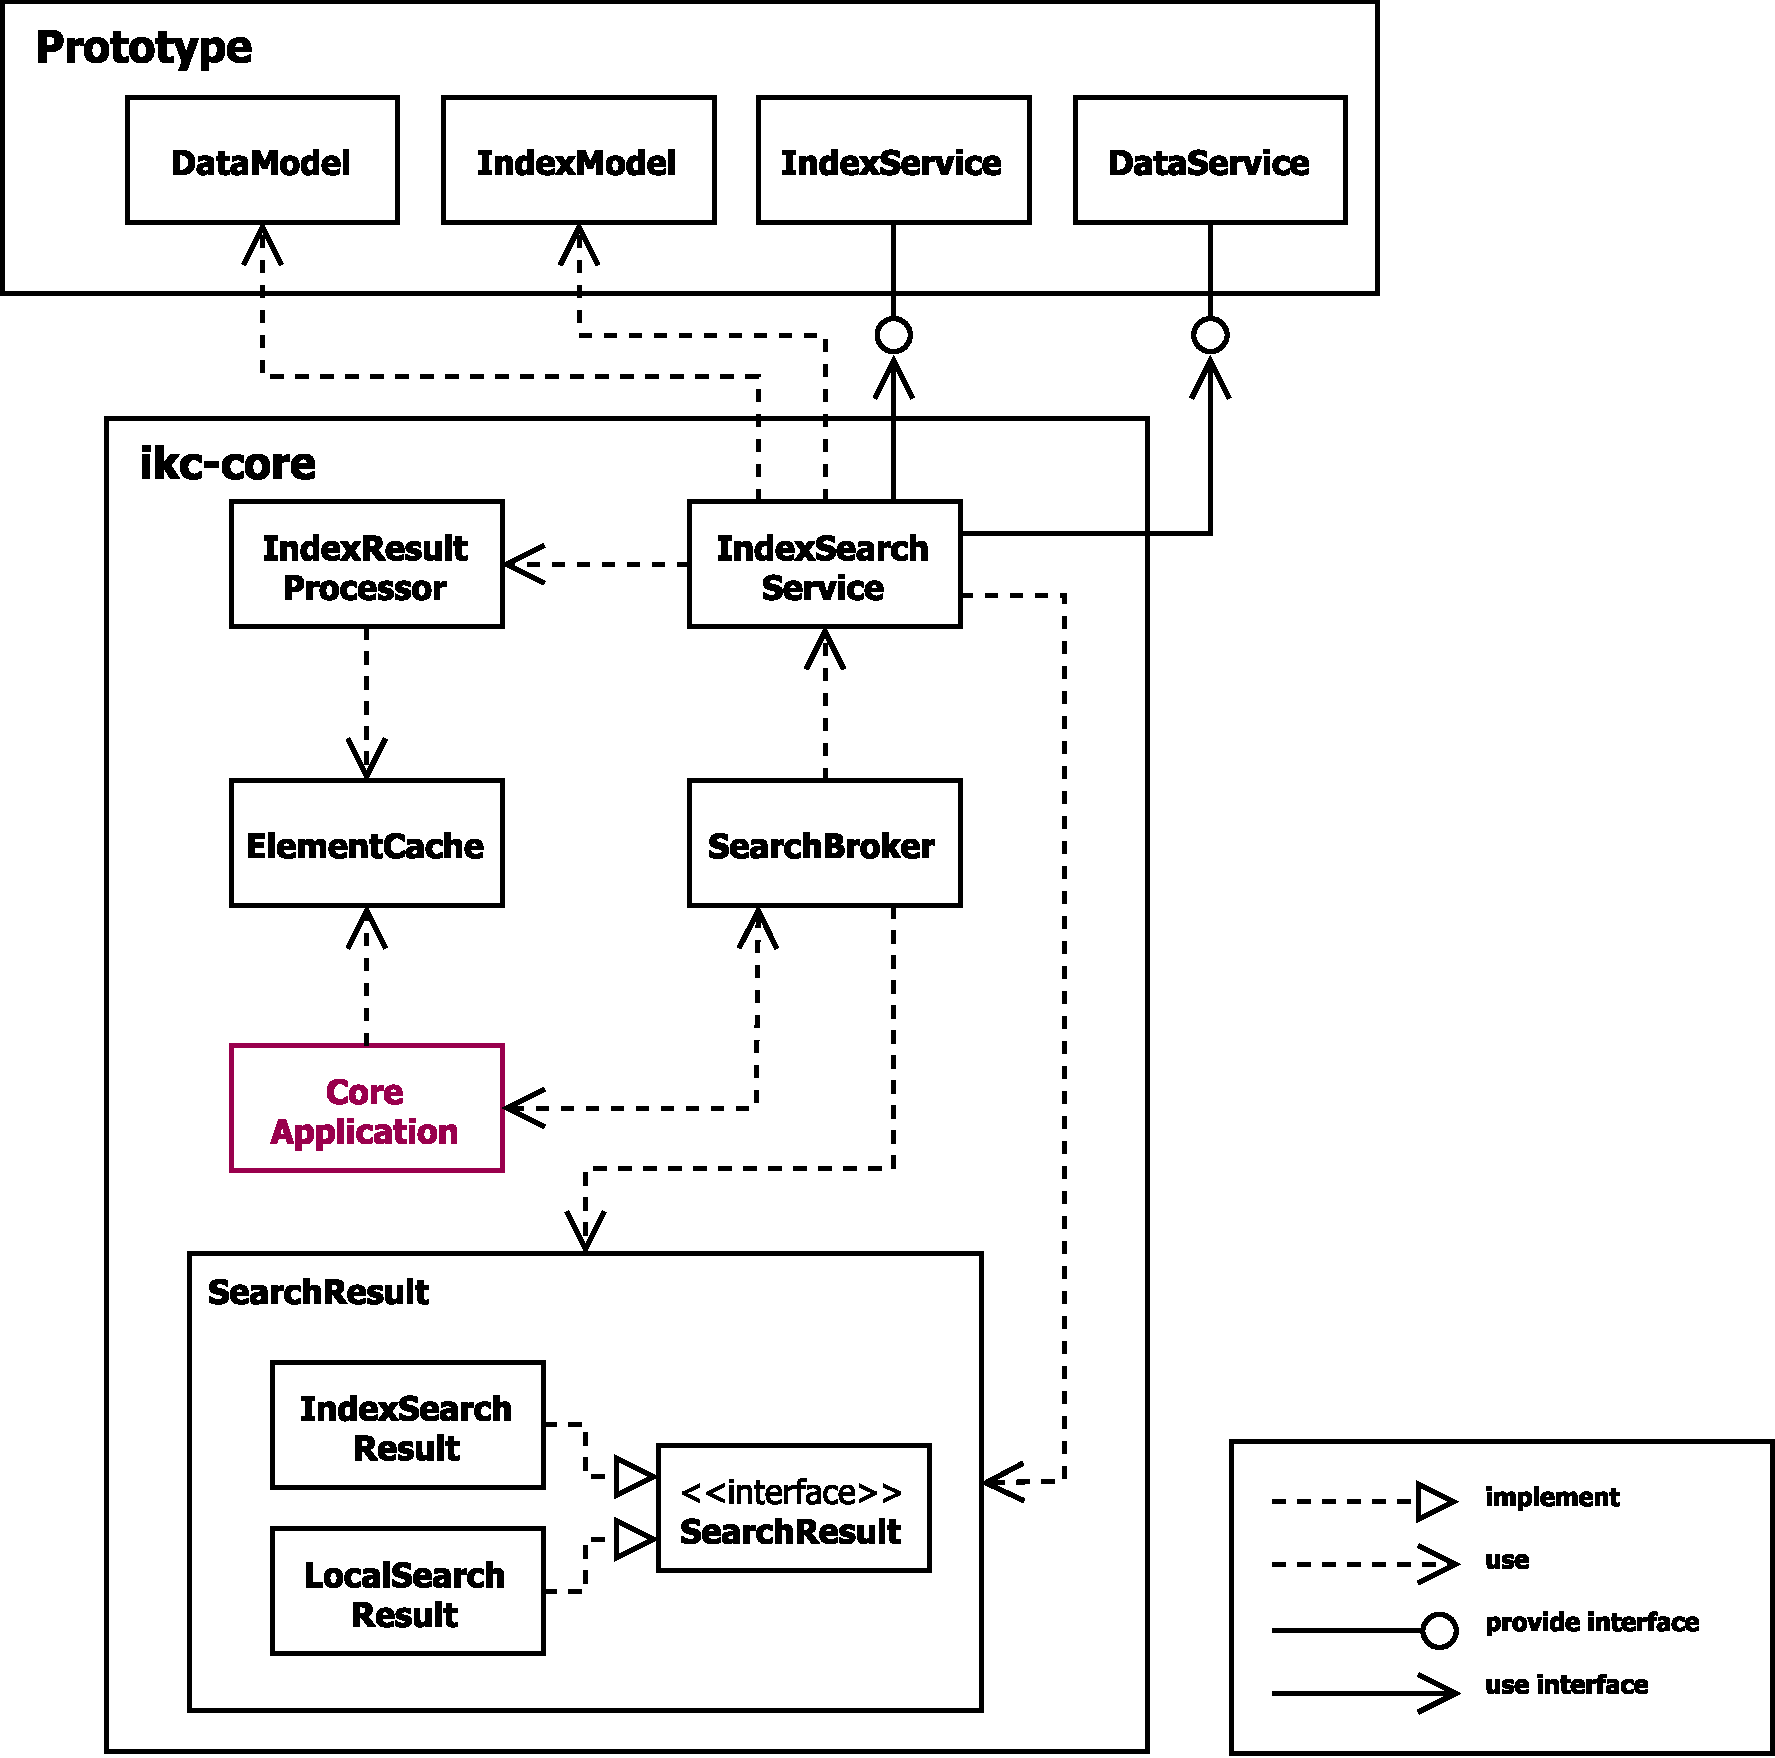
\includegraphics[width=1\textwidth]{ClassDiagrammIkcCore}
    \caption{Klassendiagramm Integration}
    \label{fig:classDiagrammIkcCore}
    \end{figure}
%riesiges index.json, ungefähr 100k Files als Text-Dateien


\subsection{Auto-Indexierung}

Da SSH Zugriff, ls -a und TimeStamp mit Map vergleichen.

    

\section{Deployment}

Die \autoref{fig:deployment-diagramm} zeigt das Deployment des \texttt{Prototypen} und des \texttt{Index}- und \texttt{Dataservices} auf in den entsprechenden Umgebungen und Services.

    \begin{figure}[H]
    \centering
    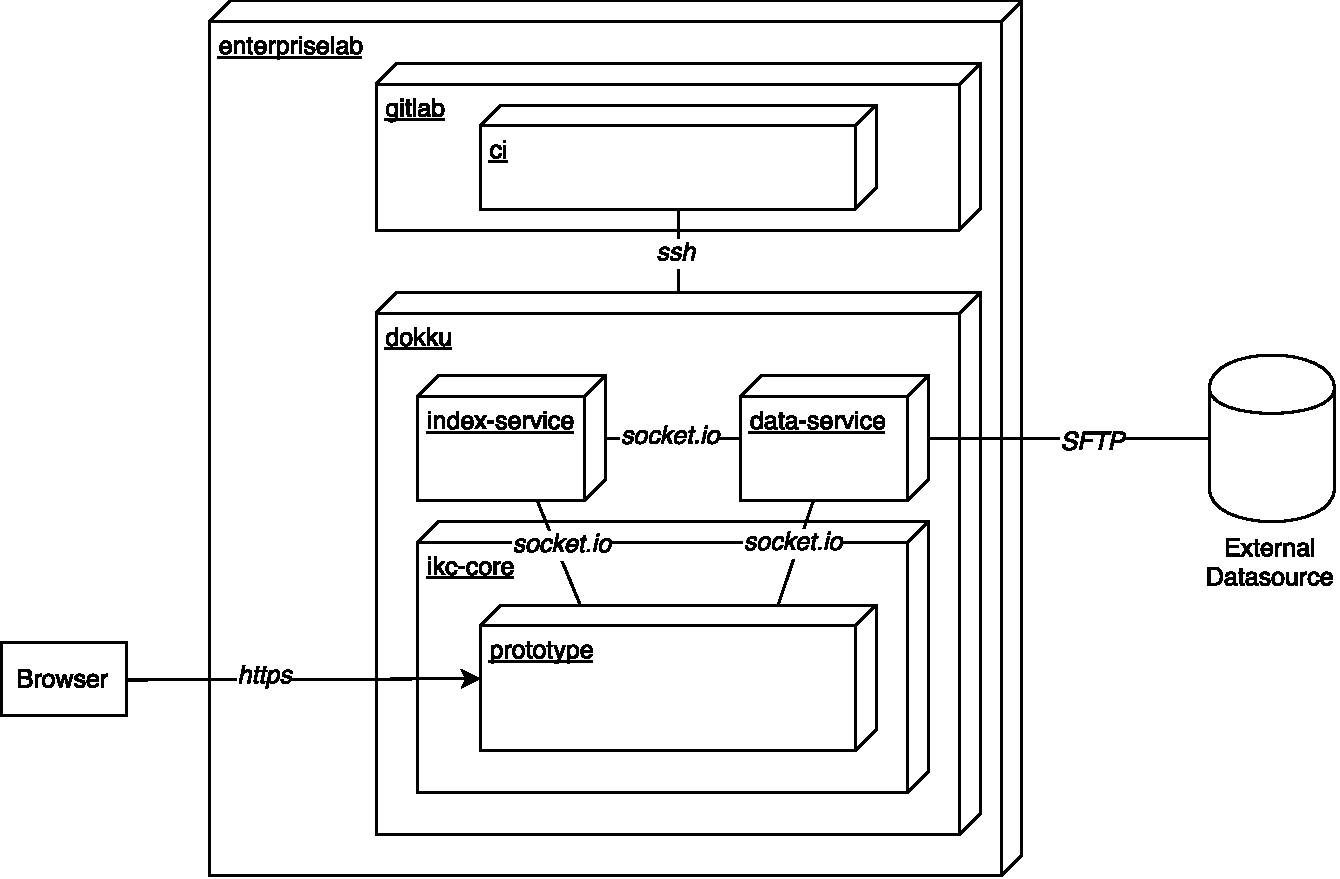
\includegraphics[width=0.8\textwidth]{DeploymentDiagramm}
    \caption{Deployment Diagramm}
    \label{fig:deployment-diagramm}
    \end{figure}

Grundsätzlich liegt jedes Projekt im \gls{gitlab} auf dem vom der Hochschule Luzern zur Verfügung gestelltem \gls{enterpriselab}. \gls{gitlab} ist eine Plattform für Versionskontrolle, Issue-Management, Continuous Integration und -Delivery oder -Deployment. Änderungen an Projekten werden ins \gls{gitlab} geladen, gebuildet und bei Erfolg direkt in eine Entwicklungs- oder Produktionsumgebung ausgeliefert.

Die Basis für die Entwicklungs- beziehungsweise Produktionsumgebungen bildet jeweils ein virtueller \gls{Ubuntu}-Server.
Prinzipiell laufen die Projekte in \gls{Docker}-Container. \gls{Dokku} erleichtert die Handhabung und den Umgang mit dem Netzwerk zusätzlich. Innerhalb vom \gls{Dokku} laufen somit die entwickelten Services wie der \texttt{Index-}, \texttt{DataService} und auch der \texttt{Prototyp}. 

Der \texttt{Prototyp} ist Teil vom bestehenden \gls{ikc-core} und wird clientseitig im Browser ausgeführt. Der \texttt{DataService} nimmt via \gls{SFTP} zusätzlich Gebrauch von einer externen Datenquelle.

\section{Benutzerhandbuch}

erwähnen und in Anhang
